\documentclass[language=en,11pt]{aghdpl}  % praca w języku angielskim

%---------------------------------------------------------------------------

\author{Kacper Rabczewski}
\shortauthor{K. Rabczewski}

\titlePL{Ulepszanie małych modeli językowych poprzez destylację łańcucha myśli}
\titleEN{Enhancing Small Language Models via Chain-of-Thought Distillation}


\shorttitlePL{Destylacja łańcucha myślowego dla małych modeli językowych}
\shorttitleEN{CoT Distillation for Small LMs}


\thesistype{Engineering Thesis}
\supervisor{Dr. Krzysztof Kluza}

\department{Department of Applied Computer Science}

\faculty{Faculty of Electrical Engineering, Automatics, Computer Science and Biomedical Engineering}

\degreeprogramme{Computer science and intelligent systems}

\date{\the\year{}}

\begin{document}
	\titlepages
	\RedefinePlainStyle

	
    \begin{abstract}
    This thesis investigates whether symbolic chain-of-thought distillation (SCoTD) can measurably improve the reasoning accuracy of a small language model on text math problems. A strong teacher model generates structured reasoning traces (CoT) for GSM8K, which are cleaned and deduplicated, and then used to finetune a 3B-class student via parameter-efficient adapters (LoRA) under 4-bit quantization. The training stack relies on modern open tooling for reproducibility and efficient use of a single 24GB GPU. Evaluation uses strict numeric exact-match parsing on GSM8K.

    Results show that SCoTD improves the student over a non-finetuned base with CoT prompting (78.54\% vs 70.51\%). A label-only variant also improves over its baseline (15.01\% vs 10.99\%), though strict formatting requirements likely undercount true ability. The teacher reaches 93.61\% on the GSM8K test split. Contributions include a cost-aware CoT data generation pipeline, a reproducible finetuning setup (LoRA + 4-bit nf4 + bf16), and an empirical analysis of accuracy, training dynamics, and operational costs. These findings support SCoTD as a practical method to enhance small models' reasoning under resource constraints.
    \end{abstract}

    \noindent\textbf{Keywords:} LLM, chain-of-thought, distillation, LoRA, QLoRA, GSM8K, reasoning, quantization

	\setcounter{tocdepth}{2}
	\tableofcontents
	\clearpage

	% \include{filename}
	\chapter{Introduction}

Large language models (LLMs) have achieved strong performance on a wide range of language tasks. However, small models (sub-4B parameters) often fall short on multi-step reasoning benchmarks such as GSM8K, where solutions require decomposing a problem into intermediate steps and computing a precise numeric answer \cite{cobbe2021trainingverifierssolvemath}. Chain-of-thought (CoT) prompting can elicit step-by-step reasoning from strong teachers and improve accuracy \cite{wei2023chainofthoughtpromptingelicitsreasoning}, especially when combined with self-consistency sampling \cite{wang2023selfconsistencyimproveschainthought}. Yet, relying on large models at inference time is costly and slow. This motivates distilling teacher reasoning traces into a small student that can run efficiently on commodity hardware.

This thesis studies supervised chain-of-thought distillation (SCoTD): a strong teacher generates structured CoTs for GSM8K questions; a small student is finetuned to reproduce these traces and final answers. The student is trained with parameter-efficient finetuning (LoRA) \cite{hu2021loralowrankadaptationlarge} on quantized weights (QLoRA) \cite{dettmers2023qloraefficientfinetuningquantized}, enabling training on a single 24GB GPU while preserving headroom to learn reasoning behavior. The approach uses standard open-source tooling for models and tokenization \cite{wolf2020huggingfacestransformersstateoftheartnatural,kudo2018sentencepiecesimplelanguageindependent,sennrich2016neuralmachinetranslationrare}.

\section*{Problem and motivation}
Small models are attractive due to their lower latency, footprint, and cost, but they struggle with multi-step math reasoning under greedy decoding. CoT distillation promises to transfer the teacher’s intermediate reasoning patterns, potentially improving student accuracy without increasing inference-time cost. The practical question is whether a 3B-class model can benefit sufficiently from SCoTD to close part of the gap to teacher performance on GSM8K.

\section*{Research questions}
\begin{itemize}
    \item RQ1: Does SCoTD improve a 3B-class model on GSM8K compared to the non-finetuned base under CoT prompting?
    \item RQ2: How does label-only supervised finetuning compare to SCoTD and base baselines under strict numeric exact-match evaluation?
\end{itemize}

\section*{Scope}
The study focuses on a single small decoder-only model (Qwen2.5-3B) \cite{qwen2025qwen25technicalreport} and a single dataset (GSM8K) \cite{cobbe2021trainingverifierssolvemath}. Teacher CoTs are produced via an API-accessible, strong reasoning model configured to emit structured steps and a line-form final answer. The student is trained with LoRA on 4-bit quantized base weights using bf16 compute, gradient checkpointing, and standard optimizers. Evaluation uses greedy decoding with strict numeric parsing; outputs that deviate from the expected format are counted as incorrect.

\section*{Contributions}
\begin{itemize}
    \item A practical, cost-aware pipeline for generating and cleaning teacher CoTs for GSM8K, with concurrency-tuned API calls and per-sample metadata for analysis.
    \item A reproducible PEFT training setup (LoRA + 4-bit nf4 + bf16) that fits on a single 24GB GPU while targeting attention and MLP projection modules.
    \item Empirical evidence that SCoTD improves a 3B-class model over base CoT prompting on GSM8K (78.54\% vs 70.51\%), with a strong teacher at 93.61\% and a label-only student that improves over baseline (15.01\% vs 10.99\%) despite strict-format penalties.
    \item Operational notes on prompt design, cleaning/deduplication, truncation policy, and evaluation pitfalls that affect measured accuracy.
\end{itemize}

\section*{Method overview}
The pipeline comprises teacher CoT generation, cleaning and deduplication, dataset processing, student finetuning (SCoTD and label-only variants), and evaluation. The student relies on PEFT with LoRA adapters \cite{hu2021loralowrankadaptationlarge} over a quantized backbone \cite{dettmers2023qloraefficientfinetuningquantized}. Tokenization is handled with a fast subword tokenizer \cite{kudo2018sentencepiecesimplelanguageindependent,sennrich2016neuralmachinetranslationrare}. Inference uses greedy decoding and a strict numeric exact-match metric. The software stack builds on Transformers and related tooling \cite{wolf2020huggingfacestransformersstateoftheartnatural}. The teacher is a strong reasoning model (DeepSeek-R1 Distill \cite{deepseekai2025deepseekr1incentivizingreasoningcapability}) accessed via OpenRouter \cite{openrouter}.

\begin{figure}[!h]
    \centering
    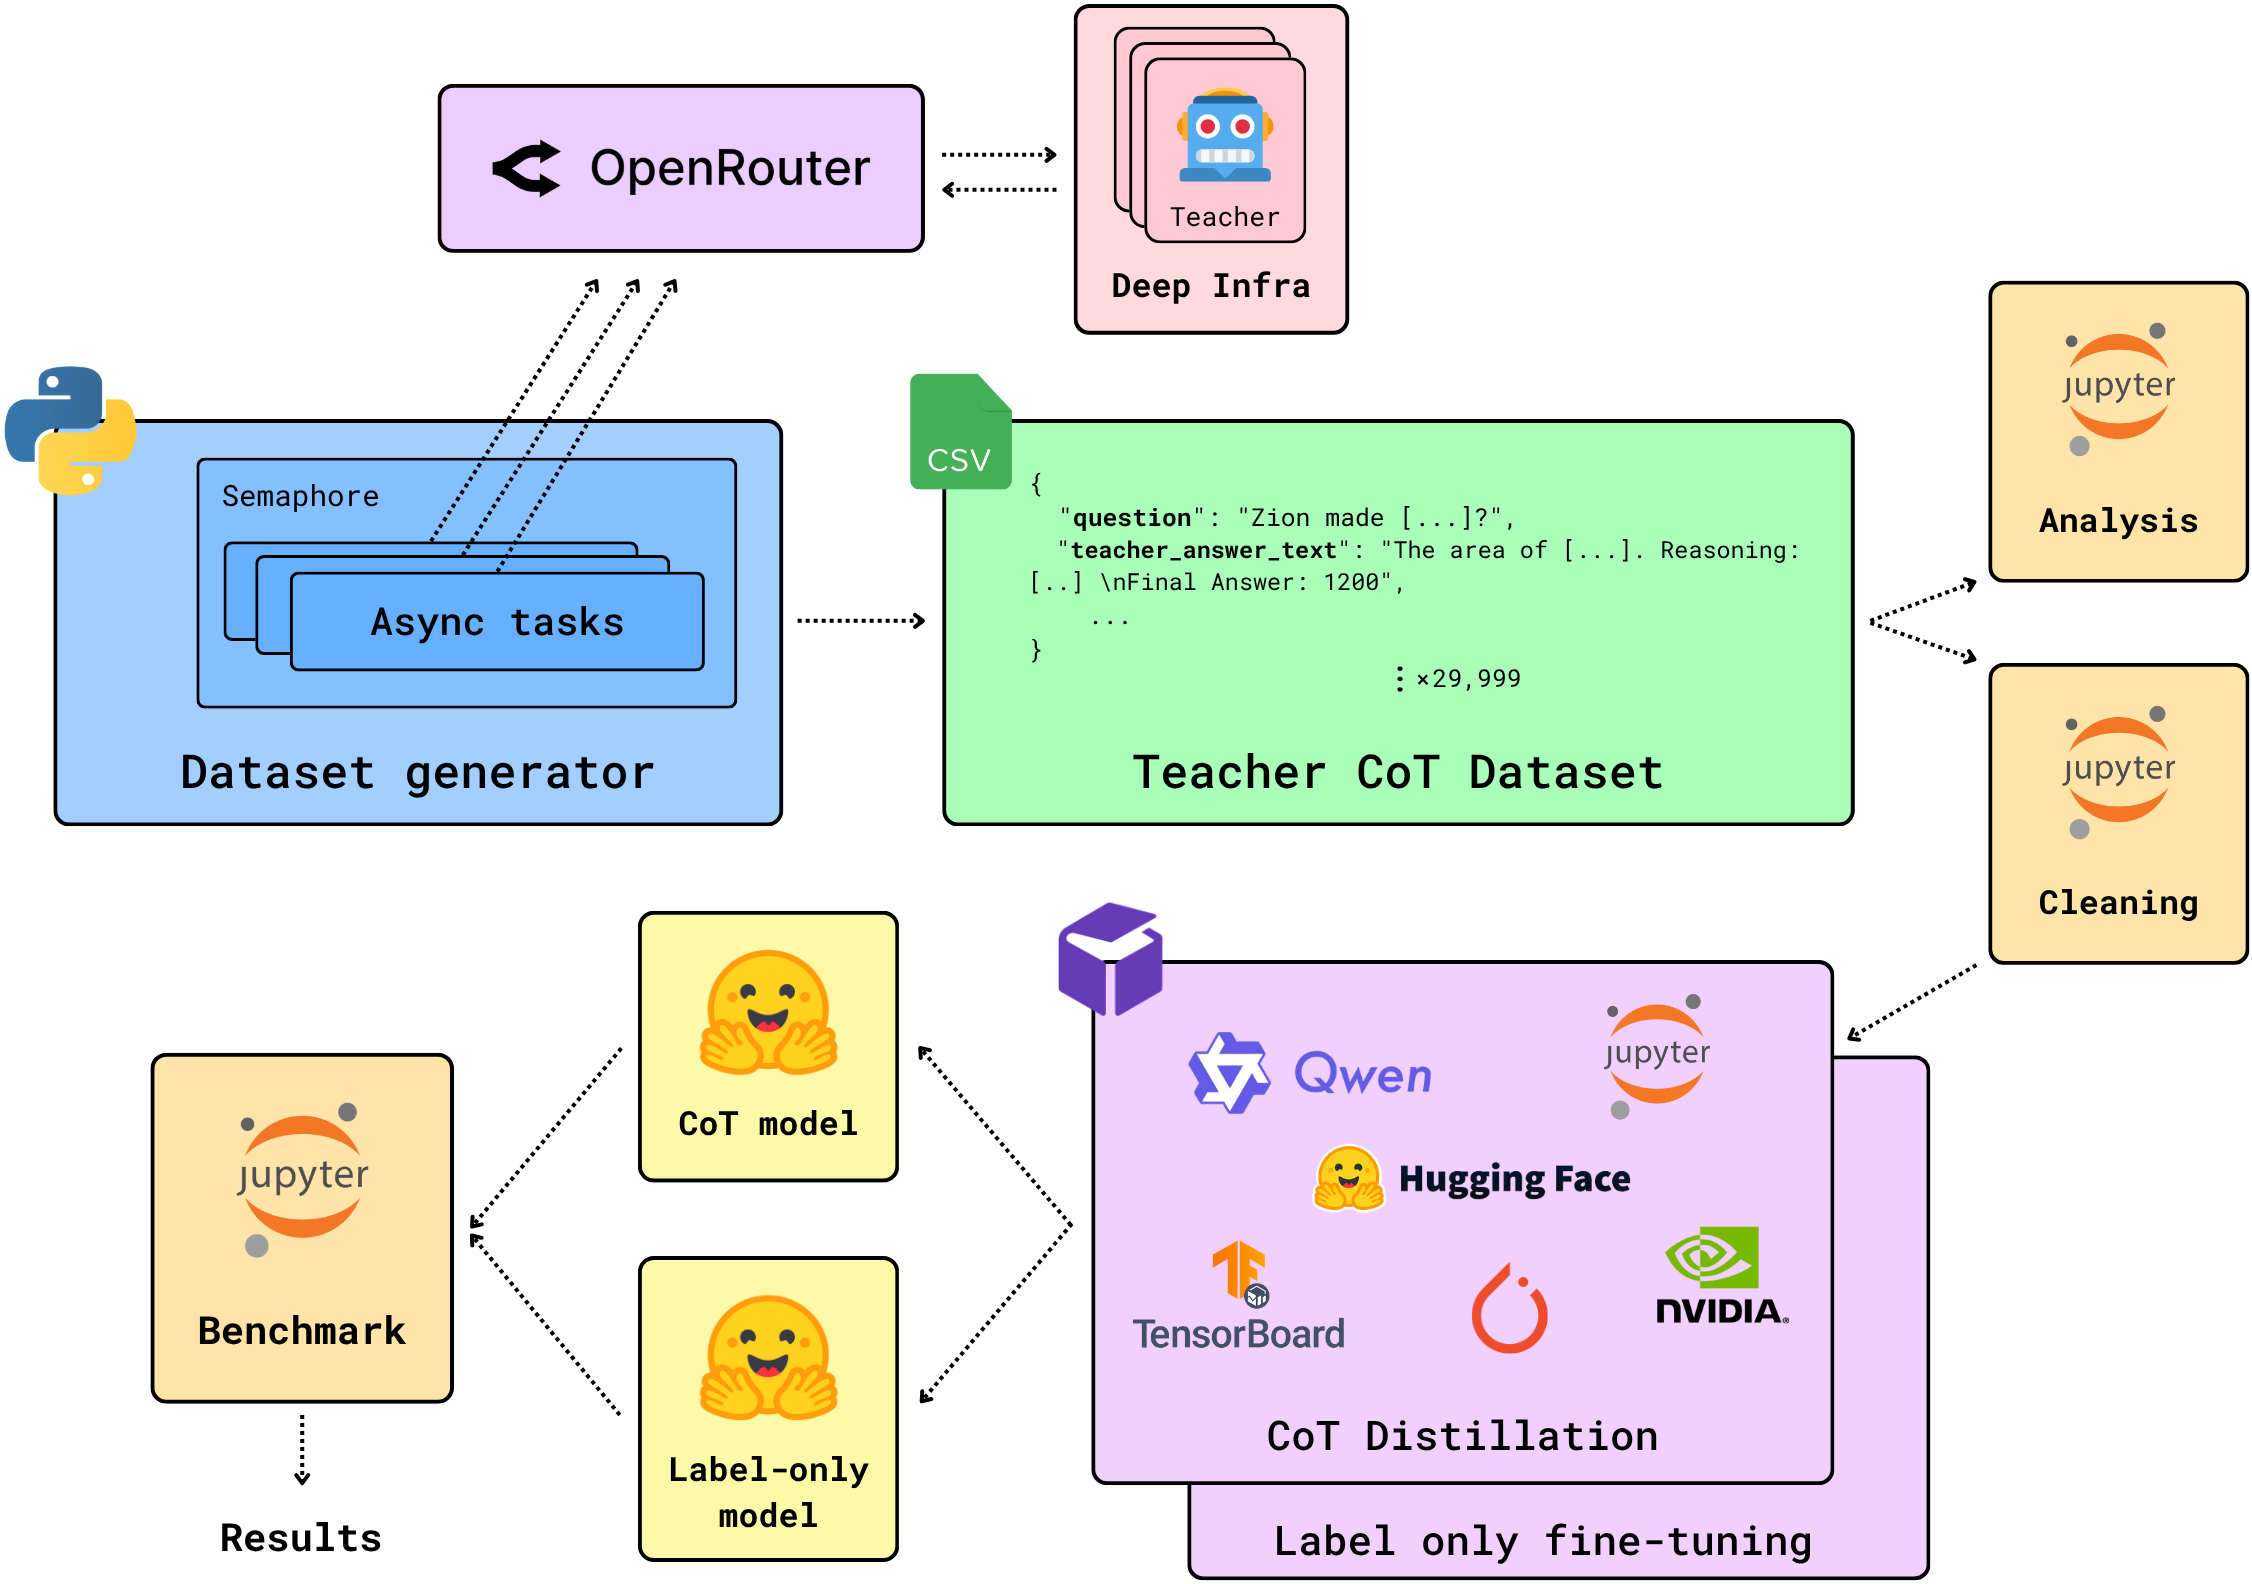
\includegraphics[width=\linewidth]{img/pipeline.png}
    \caption{End-to-end SCoTD pipeline.}
    \label{fig:pipeline-overview}
\end{figure}

\section*{Results summary}
SCoTD yields a clear gain over the base model under CoT prompting (78.54\% vs 70.51\%). Label-only finetuning improves over its baseline (15.01\% vs 10.99\%), though strict formatting likely undercounts correct numeric computations. The teacher achieves 93.61\% on GSM8K test, providing headroom and confirming the value of distilling high-quality reasoning traces.

\section*{Author background and motivation}
The author is a Co-Founder at an AI phishing detection startup that uses LLMs to analyze URLs and webpage content for malicious indicators, and a Machine Learning Engineer at OneRail building LLM-powered support workflows for same-day logistics. These roles highlighted the need for reliable, cost-efficient reasoning under tight latency and single-GPU constraints, motivating SCoTD as a practical path to higher accuracy.
	\chapter{Background}

\section{Large language models}
Large language models (LLMs) lie at the core of the current AI revolution. They are parametric probabilistic models that learn to represent the distribution of natural language sequences and generate text by autoregressively predicting one token at a time. Formally, given a tokenized sequence $(x_1, \dots, x_T)$, an LLM models $p(x_{1:T})=\prod_{t=1}^T p(x_t \mid x_{<t})$ and is trained to minimize the cross-entropy between predicted and observed tokens. LLMs derive their broad linguistic and factual knowledge from pretraining on massive text corpora using this objective, which at scale enables emergent capabilities such as in-context learning and reasoning.

\subsection{Objective and pretraining}
The standard objective is a next-token prediction:
\begin{equation}
\mathcal{L}(\theta) = - \sum_{t=1}^{T} \log p_\theta(x_t \mid x_{<t}),
\end{equation}
optimized over large, diverse datasets using gradient descent. Conceptually, this process can be understood as a vast, GPU-driven lossy compression - the model distills the statistical regularities and patterns of human language into a compact, parameterized form that enables general-purpose text understanding and generation. While pretraining is purely self-supervised, downstream adaptation may use supervised fine-tuning or preference-based methods to align behavior.

\subsection{Transformer}
Transformer architecture \cite{vaswani2023attentionneed} underlies most modern LLMs. The main building blocks are:

\begin{itemize}
    \item \textbf{Embeddings and positional encoding}: Tokens are mapped to dense vectors and augmented with position information, either sinusoidal or learned, to make the model order-aware.
    \item \textbf{Multi-head self-attention}: For each position, queries $Q$, keys $K$, and values $V$ are computed by linear projections of the hidden states. Scaled dot-product attention aggregates information across positions:
    \begin{equation}
    \mathrm{Attn}(Q,K,V) = \mathrm{softmax}\!\left(\frac{QK^{\top}}{\sqrt{d_k}}\right) V.
    \end{equation}
    Multiple heads attend in parallel to different subspaces, and their outputs are concatenated and projected.
    \item \textbf{Position-wise feed-forward network (FFN)}: A two-layer MLP with a nonlinearity (e.g., GELU) is applied independently to each position.
    \item \textbf{Residual connections and layer normalization}: Each sublayer is wrapped with residual additions and normalization for stability.
\end{itemize}

Computationally, attention has $O(L^2 d)$ time and $O(L^2)$ memory in sequence length $L$ (per batch and head factors omitted), while FFNs dominate parameter count with $O(d^2)$.

\begin{figure}[!h]
    \centering
    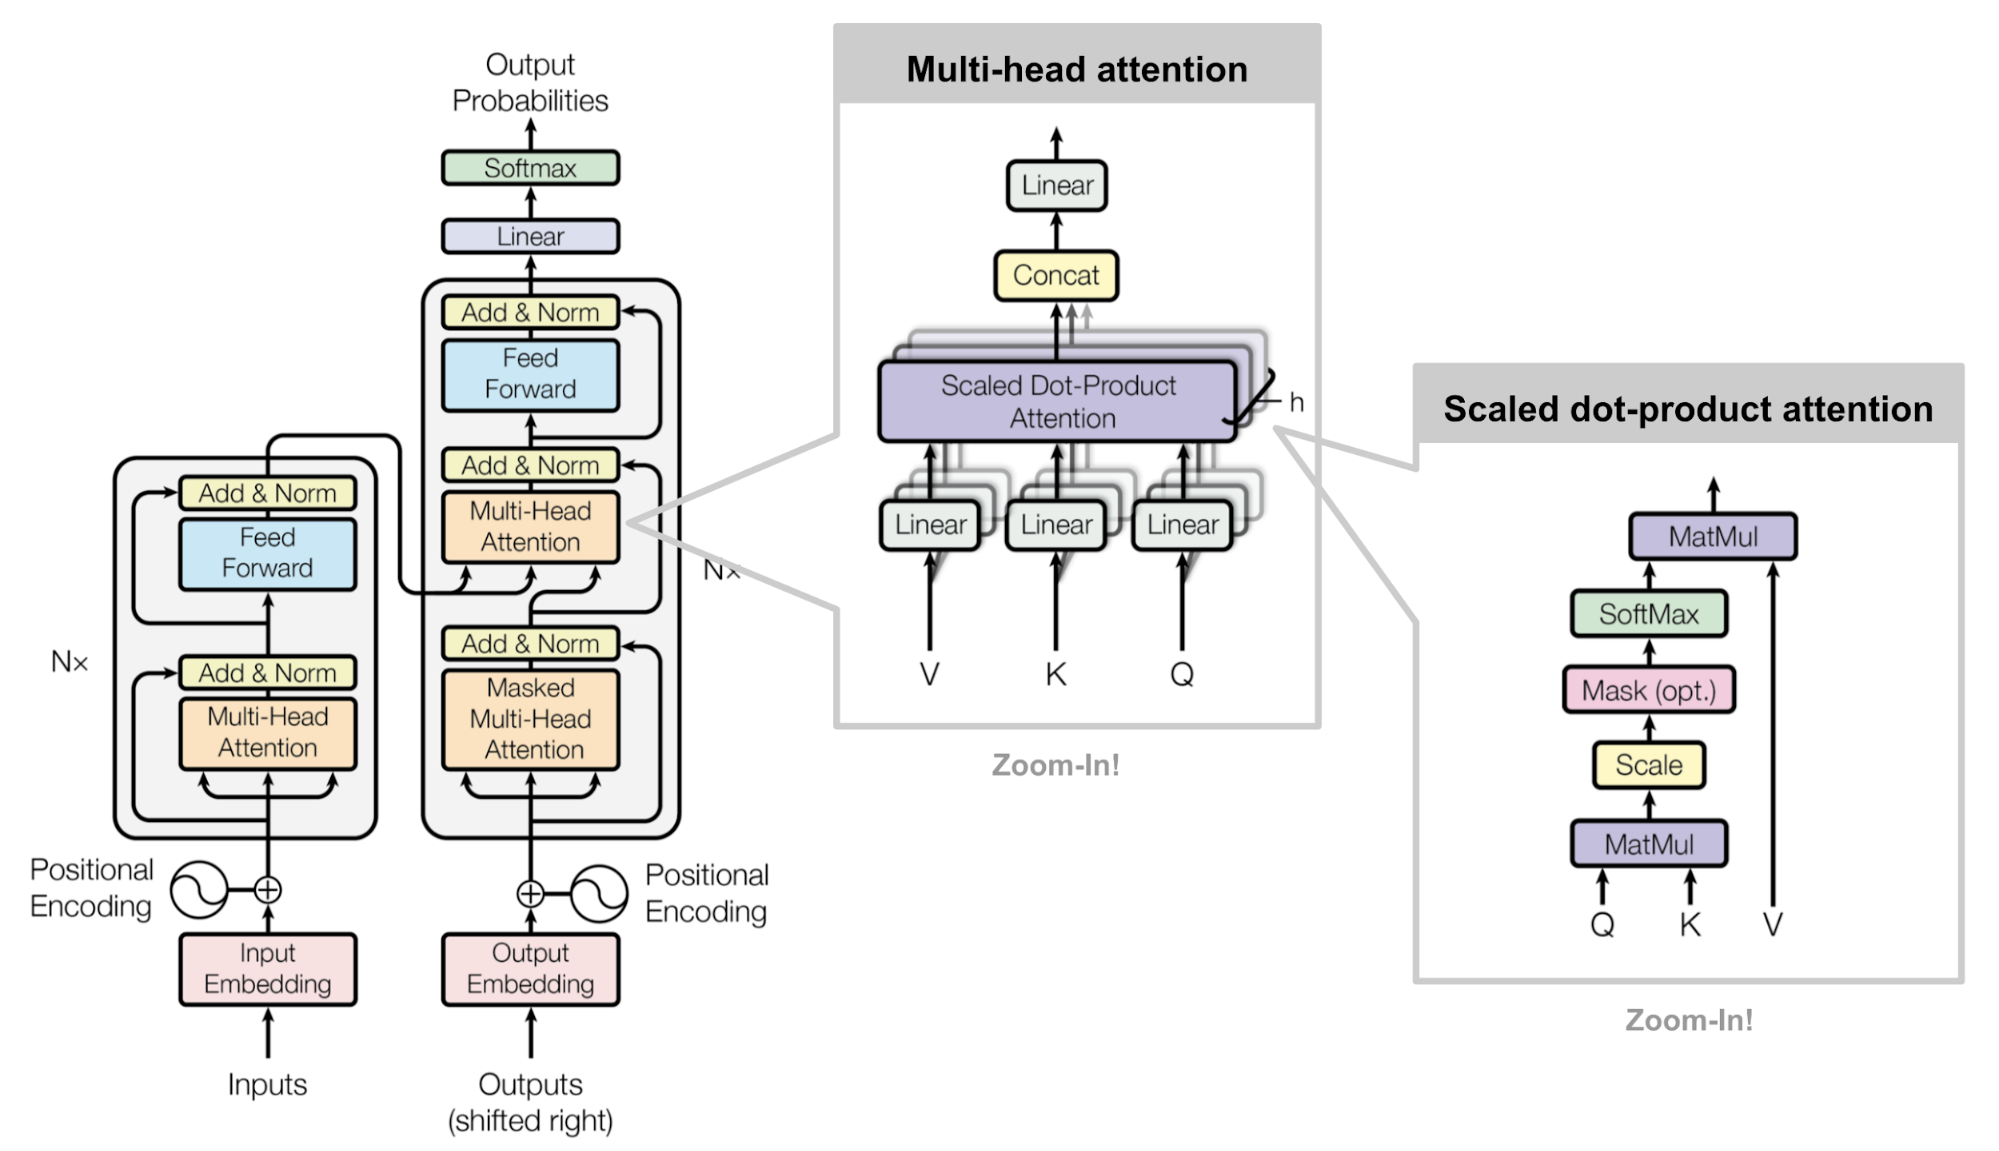
\includegraphics[width=\linewidth]{img/transformer.png}
    \caption{Transformer encoder-decoder block}
    \label{fig:transformer-block}
\end{figure}

\subsection{Decoder-only LLMs}
Decoder-only LMs use a lower-triangular mask in self-attention so that token $t$ attends only to positions $< t$. This enforces autoregressive factorization and enables left-to-right generation. During inference, key-value (KV) caching stores past projections to avoid recomputation, reducing per-token latency from quadratic to approximately linear in $L$ for attention, with constant-depth projections per layer.

\subsection{Scaling laws}
Transformers scale predictably with model size (parameters), data (tokens), and compute. Empirically, test loss follows power-law scaling with these resources \cite{kaplan2020scalinglawsneurallanguage}, implying steady gains as capacity and data increase. Practical costs rise superlinearly with size due to:

\begin{itemize}
    \item \textbf{Training}: attention's $O(L^2)$ complexity amplifies FLOPs and memory.
    \item \textbf{Inference}: latency and memory scale with depth and width; context length increases multiply attention cost without specialized kernels.
\end{itemize}

Despite costs, scaling yields emergent capabilities such as in-context learning and improved generalization \cite{brown2020languagemodelsfewshotlearners}.

\begin{figure}[!h]
    \centering
    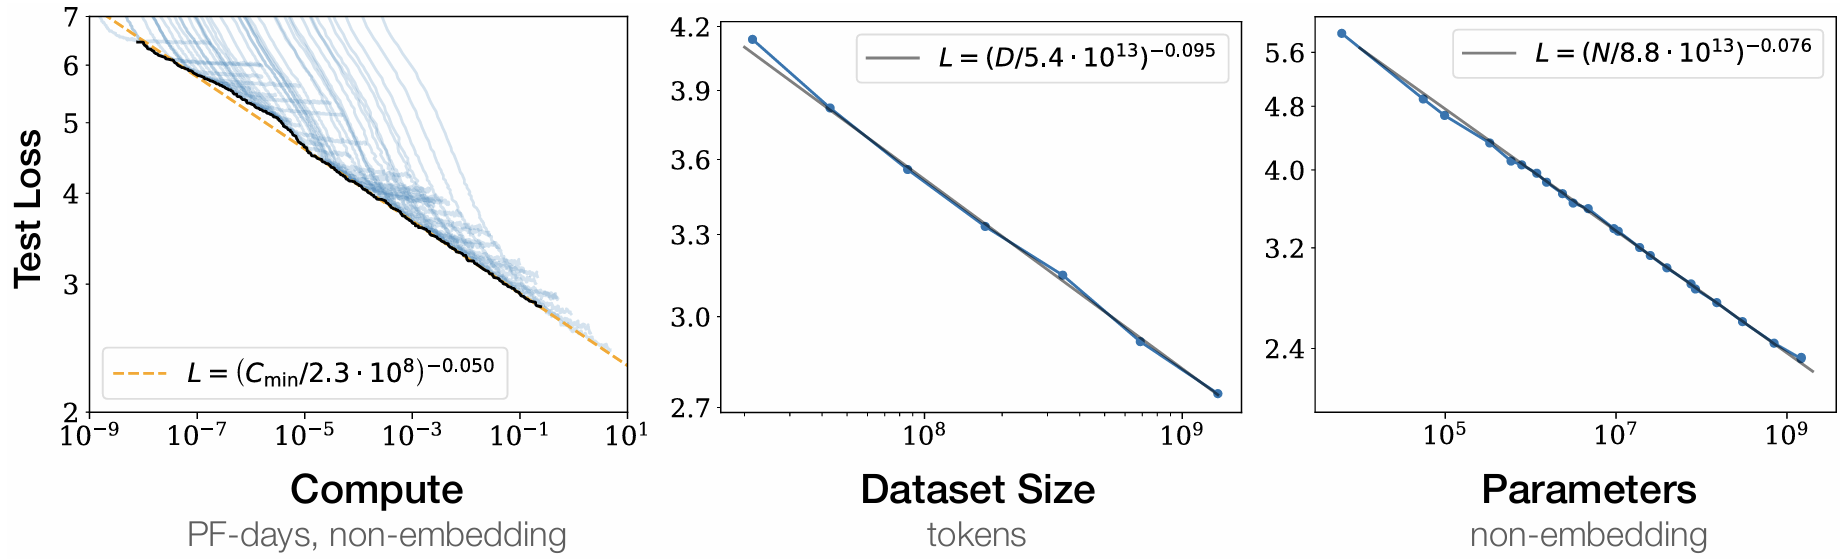
\includegraphics[width=\linewidth]{img/scaling_laws.png}
    \caption{Scaling laws: test loss vs. effective compute/model size/data on logarithmic axes.}
    \label{fig:scaling-laws}
\end{figure}

\subsection{Limitations and small-model challenges}
Large language models are known to have several limitations including:

\begin{itemize}
    \item \textbf{Hallucinations}: the model may produce fluent but unsupported statements.
    \item \textbf{Context and computation limits}: finite context windows and lack of external working memory hinder long-horizon tasks.
    \item \textbf{Compositionality}: chaining steps and maintaining intermediate variables is difficult under greedy decoding.
\end{itemize}

Small models (e.g., <4B parameters) face additional constraints which degrade multi-step arithmetic and logical reasoning, especially when strict output formats are required. While prompting and decoding strategies can mitigate some issues, structural capacity often remains the bottleneck without additional supervision or architectural support.

\section{Prompting}
Prompting is a practice of specifying a model's task through natural language. It functions as a programming interface to language models. Instruction tuning and alignment methods improve adherence to prompts \cite{ouyang2022traininglanguagemodelsfollow}.

\subsection{Paradigms}
Several prompting paradigms have emerged, often combined in practice:
\begin{itemize}
    \item \textbf{Zero-shot prompting}: The model receives only task instructions and the input. This tests inherent generalization from pretraining and any instruction tuning. It is simple and cheap but sensitive to wording and often weaker on tasks requiring intermediate computation.
    \item \textbf{Few-shot prompting}: The prompt includes $k$ input-output examples that implicitly define the task and desired format, enabling in-context learning \cite{brown2020languagemodelsfewshotlearners}.
    \item \textbf{Chain-of-Thought (CoT) prompting}: The prompt requests step-by-step reasoning, eliciting intermediate rationales before the final answer \cite{wei2023chainofthoughtpromptingelicitsreasoning}. CoT can improve complex, multi-step tasks like arithmetic by encouraging deliberate decomposition, but increases latency and token usage.
\end{itemize}

\section{Knowledge distillation}
Knowledge distillation (KD) transfers the behavior of a high-capacity teacher model to a typically smaller student \cite{hinton2015distilling}. The core idea is that softened target distributions carry "dark knowledge" about class or token similarities that hard labels do not expose, often improving generalization while enabling compression and faster inference.

\subsection{Objectives and loss design}
Response-based KD is the most widely used approach. In this setting, the student is trained to match the teacher's output distribution. Let $z^{(T)}$ and $z^{(S)}$ be teacher and student logits, and $T>0$ a temperature. The softened distributions are $p^{(T)}=\mathrm{softmax}(z^{(T)}/T)$ and $p^{(S)}=\mathrm{softmax}(z^{(S)}/T)$. A common loss combines distillation with standard supervision:
\begin{equation}
\mathcal{L} = (1-\alpha)\,\mathrm{CE}(y,\ \mathrm{softmax}(z^{(S)})) + \alpha\, T^2\, \mathrm{KL}\!\left(p^{(T)} \,\|\, p^{(S)}\right),
\end{equation}
where $y$ are hard labels and $\alpha \in [0,1]$ balances terms; the $T^2$ factor compensates for gradient scaling \cite{hinton2015distilling}.

Beyond responses, feature-based KD aligns intermediate representations (e.g., hint layers in FitNets \cite{romero2015fitnets} or attention maps in Attention Transfer \cite{zagoruyko2017paying}), while relation-based KD matches instance relations (e.g., pairwise similarities). Self-distillation trains a student from its own or a previous generation's predictions (Born-Again Networks \cite{furlanello2018bornagain}); data-augmented KD uses pseudo-labels on unlabeled data (Noisy Student \cite{xie2020noisystudent}). See \cite{gou2021survey} for a survey.

\subsection{Distillation for sequence models and LLMs}
In language modeling, KD is applied at either:

\begin{itemize}
    \item \textbf{Token level}: match teacher logits or probabilities at each decoding step, often alongside cross-entropy to the ground truth.
    \item \textbf{Sequence level}: train on sequences decoded by the teacher (e.g., beam search), simplifying the target distribution and reducing mode entropy \cite{kim2016sequence}.
\end{itemize}

Both offline (fixed teacher) and online (co-trained or periodically refreshed teacher) regimes exist. For autoregressive models, exposure bias remains; KD reduces variance but does not remove the mismatch between training and generation. Practical choices include which layers to distill, how to weight losses over time, and whether to distill only on high-confidence tokens.

\subsection{Distilling reasoning}
Symbolic Chain-of-Thought Distillation (SCoTD) transfers step-by-step reasoning from a large teacher to a smaller student by training on teacher-generated rationales rather than logits \cite{li2024symbolicchainofthoughtdistillationsmall}. Concretely: (i) curate a few-shot CoT prompt set; (ii) for each unlabeled input $x$, sample multiple CoT rationales $z$ and a prediction $y$ from the teacher; (iii) optionally filter samples to keep only label-correct pairs when gold labels are available; and (iv) fine-tune the student with the standard token-by-token language modeling objective to generate the concatenated rationale and answer. At inference, the student can decode a single rationale+answer greedily or sample multiple reasoning paths and select the majority answer via self-consistency \cite{wang2023selfconsistencyimproveschainthought}.

Empirically, SCoTD enables 125M-1.3B students to "think step-by-step"and improves accuracy on commonsense QA benchmarks (CSQA, QuaRel, OpenBookQA). A key finding is that oversampling rationales per input (e.g., $\sim$30 CoTs/example) is more important than aggressive filtering. Self-consistency particularly helps when training used noisy, unfiltered CoTs (few-shot setting), whereas its benefit diminishes once supervised filtering removes incorrect teacher answers.

\subsection{When to expect gains}
KD is most effective when the teacher's distribution contains informative structure that the student cannot infer from hard labels alone. For CoT, expected gains increase with teacher rationale quality and student capacity to model longer sequences.

\section{Parameter-efficient fine-tuning (PEFT)}
Full fine-tuning updates all model parameters and optimizer states, which scales memory, compute, and communication roughly linearly with parameter count and often requires multi-GPU setups. Optimizers like Adam maintain first and second moments, tripling memory relative to parameters alone. Checkpointing, gradient storage, and activation memory further increase requirements. Parameter-efficient fine-tuning (PEFT) alleviates these costs by freezing the backbone and training a small number of additional parameters that modulate the forward pass. This also improves modularity (task-specific heads), reduces overfitting, and enables fast switching between tasks.

\subsection{Method families}
Several PEFT families differ in where trainable parameters are introduced and how they influence the network:
\begin{itemize}
    \item \textbf{Adapters}: Small bottleneck modules (down-projection, nonlinearity, up-projection) are inserted within Transformer blocks and trained while the base model is frozen \cite{houlsby2019parameter}. They achieve near full fine-tuning performance with orders of magnitude fewer trainable parameters and support composition across tasks.
    \item \textbf{Prompt and prefix tuning}: Instead of modifying internal weights, these methods learn task-specific soft prompts. Prompt tuning optimizes a small set of embeddings prepended to the input \cite{lester2021power}, while prefix-tuning optimizes continuous key/value prefixes injected into attention at each layer \cite{li2021prefixtuning}. These approaches are extremely parameter-efficient and work well when the pretrained model already encodes the needed capabilities; performance can depend on model scale and task complexity.
    \item \textbf{Low-rank adaptation (LoRA)}: LoRA freezes the original weight matrix $W$ and parameterizes the update as a low-rank decomposition $\Delta W = A B$ with rank $r \ll \min(d_{\text{in}}, d_{\text{out}})$ \cite{hu2021loralowrankadaptationlarge}. A common scaled form is
    \begin{equation}
    W' = W + \frac{\alpha}{r}\, A B,
    \end{equation}
    where $A \in \mathbb{R}^{d_{\text{out}} \times r}$ and $B \in \mathbb{R}^{r \times d_{\text{in}}}$ are the only trainable parameters and $\alpha$ controls the update magnitude. LoRA is typically applied to attention and MLP projection matrices. Benefits include: (i) minimal trainable parameters, (ii) negligible inference overhead when merged into $W$, and (iii) modular adapters that can be stored and shared independently of the base model.
\end{itemize}

\subsection{Quantization-aware PEFT}
Quantization-aware fine-tuning combines PEFT with low-precision base weights to further reduce memory. QLoRA keeps the frozen backbone in 4-bit quantization (e.g., NF4) with per-channel scaling and "double quantization" to compress scales, while performing forward/backward compute in higher precision (e.g., bf16) and training only the PEFT parameters \cite{dettmers2023qloraefficientfinetuningquantized}. In this setup:
\begin{itemize}
    \item The quantized backbone reduces memory footprint without updating full-precision weights.
    \item LoRA (or other PEFT parameters) are maintained in higher precision and receive gradients.
    \item Careful quantizer design (NF4) and optimizer choices preserve training stability and accuracy close to full-precision baselines.
\end{itemize}
This approach enables fine-tuning larger backbones under tight memory budgets and decouples adaptation capacity (set by PEFT parameters like LoRA rank) from the storage format of the base model. Practical backends for 4-bit inference/training are widely available \cite{bitsandbytes}.

\begin{figure}[!h]
    \centering
    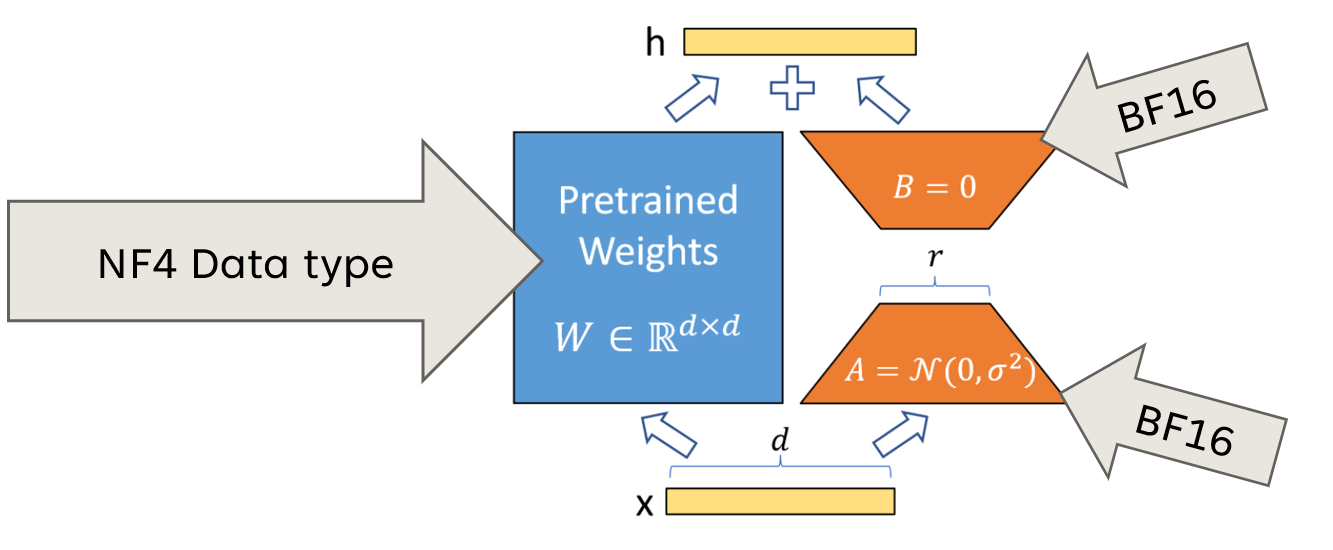
\includegraphics[width=\linewidth]{img/qlora.png}
    \caption{Model parameters under QLoRA NF4 + LoRA: frozen backbone in 4-bit quantization with per-channel scales; trainable LoRA parameters in higher precision; forward/backward compute in bf16.}
    \label{fig:qlora}
\end{figure}

\section{Tokenization}
Tokenization converts raw text into a sequence of discrete token IDs drawn from a fixed vocabulary. Language models as one of the first forward pass steps consume sequence of token IDs as input and map them to their embeddings vectors. A good scheme balances coverage (few unknowns), compact sequences (shorter length for a given text), and stability of encoding/decoding.

\subsection{Subword methods}
Pure word-level vocabularies suffer from out-of-vocabulary (OOV) issues, while character-level tokenization produces very long sequences. Subword tokenization offers a compromise by decomposing words into frequent subunits that compose to any string, including rare words and misspellings \cite{sennrich2016neuralmachinetranslationrare}.

Common approaches:
\begin{itemize}
    \item \textbf{Byte-Pair Encoding (BPE)}: the most widely used method in modern LLMs, starts from a large text corpus and iteratively merges the most frequent adjacent pairs to form larger subwords until a target vocabulary size is reached \cite{sennrich2016neuralmachinetranslationrare}. BPE yields deterministic segmentations given the learned merges and has no explicit probabilistic model.
    \item \textbf{WordPiece}: subword units to maximize likelihood of a training corpus, typically under a simple probabilistic model over segmentations; greedy decoding selects the best segmentation. It typically includes reserved continuation markers to indicate that a subword is not word-initial.
    \item \textbf{SentencePiece}: optimizes a probabilistic unigram model over a candidate subword inventory and prunes units that hurt likelihood \cite{kudo2018sentencepiecesimplelanguageindependent}. It supports sampling alternative segmentations during training for robustness and can operate directly on raw text without external pre-tokenization.
\end{itemize}

Implementation frameworks such as SentencePiece and Transformers provide standardized training, encoding, and decoding pipelines \cite{kudo2018sentencepiecesimplelanguageindependent,wolf2020huggingfacestransformersstateoftheartnatural}. Variants like byte-level BPE ensure coverage of arbitrary Unicode by operating on UTF-8 bytes, which removes true OOVs at the cost of sometimes longer sequences for non-Latin scripts.

\begin{figure}[t]
    \centering
    \includegraphics[width=\linewidth]{figures/tokenization-examples.pdf}
    \caption{Tokenization }
    \label{fig:tokenization-examples}
\end{figure}

\subsubsection{Vocabulary}
Larger token vocabularies can represent up to whole words, reducing sequence length and attention cost. However, they implicitly increase embedding and output layer sizes, memory, and may cause overfitting. Smaller vocabularies generalize better to rare forms but inflate sequence length, which increases quadratic attention cost and risk of truncation. Practical choices range from 16k-200k subwords.

\subsubsection{Normalization and pre-tokenization.}
Many pipelines normalize text (e.g., Unicode NFKC, lowercasing, whitespace handling) to improve robustness; SentencePiece can integrate normalization and avoid external word boundary rules \cite{kudo2018sentencepiecesimplelanguageindependent}. Pre-tokenizers may split on whitespace and punctuation to enforce word boundary awareness before applying subword merges. Choices here affect how punctuation, casing, and whitespace survive round-trip detokenization.

\subsection{Special tokens and sequence framing}
Special tokens mark structure and control decoding:
\begin{itemize}
    \item \textbf{BOS/EOS}: Begin-of-sequence and end-of-sequence delimit the sequence and signal termination.
    \item \textbf{PAD}: Padding aligns sequences within a batch to a common length; attention masks ensure pads are ignored during loss computation and attention.
    \item \textbf{Instruction tokens}: Special markers that indicate task boundaries or specify desired behavior (e.g., \texttt{<|user|>}, \texttt{<|assistant|>}, \texttt{<|thought|>}).
\end{itemize}
Figure~\ref{fig:sequence-framing} shows the instruction/assistant turn framing and BOS/EOS/PAD usage.

\begin{figure}[t]
    \centering
    \includegraphics[width=\linewidth]{figures/sequence-framing.pdf}
    \caption{Sequence framing with special tokens: example instruction–response turns using BOS/EOS and task-specific role tokens (e.g., <|user|>, <|assistant|>).}
    \label{fig:sequence-framing}
\end{figure}

\section{GSM8K}
GSM8K is a benchmark of 8.5K English grade-school math word problems designed to evaluate multi-step reasoning in natural language \cite{cobbe2021trainingverifierssolvemath}. Problems typically require 2-8 steps of elementary arithmetic ($+,-,\times,\div$) and include human-written, natural-language solutions with inline ``calculator annotations'' (intermediate computations) and a final integer answer on a separate line. The benchmark is widely used to study prompting and reasoning supervision; standard scoring is exact numeric match, often evaluated under chain-of-thought prompting and self-consistency sampling \cite{wei2023chainofthoughtpromptingelicitsreasoning,wang2023selfconsistencyimproveschainthought}.

\subsection{Dataset overview and structure}
Released in English via HuggingFace Datasets \cite{lhoest2021datasetscommunitylibrarynatural}, GSM8K provides two configurations: a main set (question, rationale, final answer) and a socratic variant that interleaves sub-questions within the solution. Official splits comprise 7{,}473 training and 1{,}319 test problems \cite{cobbe2021trainingverifierssolvemath}; each instance pairs a question string with a multi-step natural-language solution containing intermediate calculations and a single integer final answer.
Figure~\ref{fig:gsm8k-example} shows an example question, rationale with inline calculations, and final integer answer line.

\begin{figure}[t]
    \centering
    \includegraphics[width=\linewidth]{figures/gsm8k-example.pdf}
    \caption{GSM8K example: (left) problem statement; (right) step-by-step rationale with calculator-style intermediate computations, followed by a final integer answer on its own line.}
    \label{fig:gsm8k-example}
\end{figure}
	\chapter{Methodology}

\section{System requirements}

\subsection{Functional requirements}
\begin{itemize}
    \item Generate a sufficiently large, high-quality, correctly answered set of teacher CoT samples for a GSM8K training subset.
    \item Persist per-sample metadata (latency, token counts, correctness, cost) for analysis.
    \item Fine-tune a single small student model to emit coherent step-by-step reasoning and a correctly formatted final answer line.
    \item Fine-tune a single small student model to emit only the correctly formatted final answer line.
    \item Evaluate all models (base, students, teacher) on the GSM8K test split under strict numeric exact-match parsing of the final answer line.
\end{itemize}

\subsection{Non-functional requirements}
\begin{itemize}
    \item \textbf{Optimized asynchronous generation}: Highly asynchronous dataset generator with concurrency tuned to balance throughput and timeout/error rate.
    \item \textbf{Observability}: Persistent logging of token usage, latency distributions, and derived cost metrics during dataset generation.
    \item \textbf{Data quality}: Diverse and coherent chain-of-thought reasoning. Removal of outliers.
    \item \textbf{Resource efficiency}: All training and benchmarking runs fit in available VRAM without OOM.
    \item \textbf{Format compliance}: Final answer line must follow ``Final Answer: <integer>'' exactly. Deviation counts as failure.
    \item \textbf{Maintainability}: Separation of data generation, cleaning, training, and evaluation stages with clear artifact boundaries.
    \item \textbf{Reproducibility}: Deterministic training pipeline, versioned artifacts, prompts, configuration, environment and scripts.
    \item \textbf{Budget adherence}: Monitor spend so teacher generation and GPU usage stay within the stated cap.
\end{itemize}

\subsection{Constraints}
\begin{itemize}
    \item Single-GPU environment - no multi-node or distributed training.
    \item Fixed public benchmark - GSM8K.
    \item Teacher accessed only via external API.
    \item Limited sequence context - excessive rationales must be pruned or truncated without losing the final answer line.
    \item Budget cap at 200\,PLN.
\end{itemize}

\subsection{Success criteria}
\begin{itemize}
    \item Accuracy improvement of the distilled student over the base CoT-prompted model by at least 5 percentage points on GSM8K test.
    \item Cleaned dataset size sufficient to enable measurable gains (tens of thousands of rationale+answer pairs) without exceeding resource limits.
    \item All runs complete within available GPU memory and budget envelope.
\end{itemize}

\subsection{Risks and mitigation}
\begin{itemize}
    \item \textbf{Overfitting to limited subset}: Mitigate via data augmentation and training regularization.
    \item \textbf{Format consistency}: Enforce prompt templates and validation during evaluation.
    \item \textbf{Data noise leakage}: Strict filtering to remove incorrect teacher answers before student training.
    \item \textbf{Cost escalation}: Concurrency and request budgeting monitored. Setting account balance limits for GPU usage.
\end{itemize}

\section{Architecture}
The system is an offline teacher-to-student pipeline that produces a cleaned CoT dataset and trains a 3B-class student with PEFT, then evaluates under strict numeric exact match.

\subsection{Components}
\begin{itemize}
    \item \textbf{Teacher generator}: Async OpenRouter client producing structured CoTs.
    \item \textbf{Prompts/config}: Versioned templates under \texttt{prompts/} with a meta JSON capturing decoding + generation config.
    \item \textbf{Dataset artifacts}: Raw, cleaned, and processed JSONL stages (introduced once in Data Flow).
    \item \textbf{Cleaning \& preprocessing}: Notebooks applying correctness filtering, rationale dedup, and length outlier removal.
    \item \textbf{Training}: Notebook performing QLoRA fine-tuning of two modes (SCoTD and label-only).
    \item \textbf{Evaluation}: Notebook for greedy exact-match benchmarking.
    \item \textbf{Runtime}: Single Python environment.
\end{itemize}

\subsection{Data flow}
\begin{enumerate}
    \item \textbf{Ingest}: Load GSM8K train/test splits; select first $\sim$1{,}000 train questions.
    \item \textbf{Generate}: Oversample $\sim$30 CoTs per question asynchronously and write raw JSONL.
    \item \textbf{Clean}: Apply correctness filter, rationale dedup, and 99th percentile length trimming and produce cleaned JSONL.
    \item \textbf{Process}: Project cleaned dataset to minimal supervised learning schema and produce processed JSONL.
    \item \textbf{Train}: Two modes (SCoTD, label-only).
    \item \textbf{Evaluate}: Strict numeric exact-match benchmarking.
\end{enumerate}

\section{Teacher CoT dataset generation}
This stage produces a cleaned high-quality rationale+answer corpus from a strong reasoning model.

\subsection{Subset selection}
For cost control only the first $\sim$1{,}000 GSM8K train questions are used. Each question targets 30 samples (oversampling for rationale diversity). Generation is resumable: existing \texttt{(question\_id, sample\_id)} pairs found in the output JSONL are skipped on subsequent runs.

\subsection{Async generation}
An async Python client (HTTPX) calls the OpenRouter \texttt{/chat/completions} endpoint for model \texttt{deepseek/deepseek-r1-distill-qwen-32b}. Concurrency is capped at 25 via an \texttt{asyncio.Semaphore}. Each request includes:
\begin{itemize}
    \item System prompt: concise reasoning format specification.
    \item User prompt: templated few-shot exemplars + target question.
    \item Decoding: \texttt{temperature=1.0}, \texttt{top\_p=1.0}.
    \item Timeout: 120\,s.
\end{itemize}

Tenacity applies exponential backoff (max 5 attempts) on transport errors.

\subsection{Formatting contract}
Required output:
\begin{verbatim}
Reasoning:
- step 1
- step 2
...
Final Answer: <number>
\end{verbatim}
No extra trailing text. Final line must start exactly with \texttt{Final Answer:}. Parser scans lines to extract the numeric suffix.

\subsection{Parsing and correctness}
\begin{itemize}
    \item Gold answer number: extracted from GSM8K \texttt{answer} field after the \texttt{####} delimiter using a final-number regex.
    \item Teacher answer number: last numeric token on the \texttt{Final Answer:} line (regex supports integers, decimals, scientific notation).
    \item Correctness: strict numeric equality (Python int/float comparison). Any parsing failure or missing final line marks the sample invalid (counted as failed).
\end{itemize}

\subsection{Recording schema}
Each raw sample appended as a JSONL record with fields:
\texttt{question\_id, sample\_id, question, gold\_answer\_text, gold\_answer\_number, teacher\_answer\_text, teacher\_answer\_number, is\_correct, finish\_reason, usage\{prompt\_tokens, completion\_tokens\}, latency\_ms, model, request\_id}. Latency is wall-clock from request dispatch to response receipt.

\subsection{Resumability}
Before generating new samples, existing JSONL is scanned to build a per-question set of occupied \texttt{sample\_id}s. Missing IDs in \([0, N)\) are generated where completed questions are skipped entirely.

\subsection{Progress and metrics}
A live tqdm progress bar displays:
\begin{itemize}
    \item \textbf{cost}: computed continuously as
    \[
      \text{cost} = \frac{T_{in}}{10^6} c_{in} + \frac{T_{out}}{10^6} c_{out}
    \]
    with $c_{in}=c_{out}=\$0.27$/M tokens (taken from OpenRouter).
    \item \textbf{tokens\_in / tokens\_out}: cumulative prompt / completion tokens.
    \item \textbf{acc}: running fraction of \texttt{correct\_samples / total\_samples}.
    \item \textbf{ok/err}: successful vs failed attempts.
\end{itemize}

\subsection{Failure handling}
Failures include HTTP errors, timeouts, parsing errors, or malformed responses. Each increments \texttt{failed\_samples} and no partial record is written. Retries only cover transport exceptions—logical format violations are not retried to avoid cost inflation.

\subsection{Quality outcome}
Oversampling plus strict filtering yields a pool of diverse, correctly formatted rationales per question (typically multiple distinct reasoning paths). This supports effective downstream distillation while keeping total spend within the budget envelope.

\section{Cleaning}
This stage removes incorrect, duplicate, and extreme-length samples to yield a high-signal supervision set.

\subsection{Input}
Raw JSONL: \texttt{artifacts/data/raw/dataset.jsonl} containing 30{,}000 generations (1{,}000 questions $\times$ 30 samples), each with correctness flag, usage tokens, and rationale text.

\subsection{Operations}
\begin{enumerate}
    \item \textbf{Load \& index}: Read JSONL into a DataFrame indexed by \texttt{(question\_id, sample\_id)} for deterministic ordering.
    \item \textbf{Correctness filter}: Keep only rows where \texttt{is\_correct = True}. Removes all teacher numeric mismatches; prevents label noise (primary gain).
    \item \textbf{Exact rationale dedup}: Drop duplicates on \texttt{teacher\_answer\_text}. Prevents overweighting identical reasoning paths.
    \item \textbf{Token-length outlier removal}: Compute per-row \texttt{total\_tokens = prompt\_tokens + completion\_tokens}. Remove rows with \texttt{total\_tokens} $\ge$ 99th percentile (threshold 1392 tokens). This trims extreme verbose rationales that inflate sequence length and memory without adding diversity.
    \item \textbf{Persist}: Reset index and write cleaned JSONL to \texttt{artifacts/data/cleaned/dataset.jsonl}.
\end{enumerate}

\subsection{Justification}
\begin{itemize}
    \item \textbf{Strict correctness}: Ensures the student never trains on wrong final answers (no noisy label memorization).
    \item \textbf{Deduplication}: Reduces redundant gradient steps; improves effective rationale variety per batch.
    \item \textbf{Length capping}: Controls worst-case sequence length to avoid GPU OOM and keeps average tokens closer to the median (739 total tokens).
\end{itemize}

\subsection{Outcome}
Resulting size: 24{,}952 cleaned samples (from 30k raw). Teacher correctness in retained set is 100\%. Distribution tails (>\,99th percentile) removed while preserving all final answer lines.

\section{Preprocessing}
Transforms the cleaned corpus into the minimal supervision schema consumed by training scripts.

\subsection{Input}
Cleaned JSONL: \texttt{artifacts/data/cleaned/dataset.jsonl} (indexed by \texttt{question\_id}, \texttt{sample\_id}).

\subsection{Output}
Select only: \texttt{question}, \texttt{gold\_answer\_text}, \texttt{gold\_answer\_number}, \texttt{teacher\_answer\_text} \quad (rationale + final answer line), \texttt{teacher\_answer\_number}
Index columns are preserved until final write, then flattened.

\subsection{Artifact}
Write to \texttt{artifacts/data/processed/dataset.jsonl}.

\subsection{Schema Rationale}
Minimal fields reduce I/O and memory footprint, remove unused metadata (latency, token usage) for training, and keep both textual and numeric answers to enable strict evaluation parsing and auxiliary checks.

\subsection{Integrity}
All records already passed strict correctness; no further validation required. Numeric fields (\texttt{gold\_answer\_number}, \texttt{teacher\_answer\_number}) support exact-match evaluation; textual rationale preserved verbatim for supervised reasoning.

\section{Prompt templates}\label{sec:prompt_templates}
This section touches on the fixed prompt templates used across generation, training, and benchmarking. Templates are versioned as plain text under \texttt{code/prompts/}. No runtime mutation other than \texttt{\{question\}} placeholder replacement.

\subsection{Files and roles}
\begin{itemize}
    \item \textbf{CoT system} (\texttt{code/prompts/cot/system.txt}): Instructs concise multi-step reasoning (2--8 steps) plus a terminating final answer line.
    \item \textbf{CoT user} (\texttt{code/prompts/cot/user.txt}): Provides three few-shot exemplars (question, reasoning steps, final answer) followed by the target question placeholder.
    \item \textbf{Label-only system} (\texttt{code/prompts/label\_only/system.txt}): Constrains output to a single final answer line with no reasoning.
    \item \textbf{Label-only user} (\texttt{code/prompts/label\_only/user.txt}): Supplies same three few-shot answer-only exemplars plus the target question placeholder.
\end{itemize}

\subsection{Formatting contracts}
\begin{itemize}
    \item \textbf{CoT prompts}: 
    \begin{verbatim}
Reasoning:
- step 1
- step 2
...
Final Answer: <number>
    \end{verbatim}
    2--8 dash-prefixed steps; arithmetic shown explicitly; no trailing text after the final answer line.
    \item \textbf{Label-only prompts}: Single line \texttt{Final Answer: <number>} No units, commentary, or extra lines.
\end{itemize}

\section{Training}
Goal of training is to fine-tune a single 3B decoder-only model (Qwen/Qwen2.5-3B) with QLoRA under 4-bit NF4 quantization and LoRA adapters, using bfloat16 precision.

\subsection{Model, quantization, and PEFT}
\begin{itemize}
    \item Base: \texttt{Qwen/Qwen2.5-3B} loaded with BitsAndBytes 4-bit (\texttt{nf4}, double-quantization), compute dtype bf16; \texttt{device\_map="auto"}.
    \item Gradient checkpointing enabled; \texttt{model.config.use\_cache = false} during training.
    \item Tokenizer: fast; if \texttt{pad\_token} is missing, set to \texttt{eos\_token} and propagate pad IDs to model and generation config.
    \item LoRA: \texttt{r=16}, \texttt{alpha=32}, \texttt{dropout=0.05}, \texttt{bias="none"} on \{\texttt{q\_proj}, \texttt{k\_proj}, \texttt{v\_proj}, \texttt{o\_proj}, \texttt{gate\_proj}, \texttt{up\_proj}, \texttt{down\_proj}\}; task type \texttt{CAUSAL\_LM}.
\end{itemize}

\subsection{Data split and reproducibility}
\begin{itemize}
    \item Input: \texttt{artifacts/data/processed/dataset.jsonl}.
    \item Split: 80/20 by \texttt{question\_id} (\texttt{TRAIN\_SPLIT=0.8}) with \texttt{seed=42} ensures no question leakage across splits.
    \item Label-only mode dedup: keep a single record per \texttt{question\_id} (first by \texttt{sample\_id}) to avoid multiple labels per question.
    \item Seeds for Python, PyTorch, CUDA, and accelerate set to 42; TF32 enabled on matmul/CuDNN.
\end{itemize}

\subsection{Prompting and target formatting}
\begin{itemize}
    \item Prompts: training/inference use the same templates.
    \begin{itemize}
        \item SCoTD: \texttt{prompts/cot/system.txt} + \texttt{prompts/cot/user.txt}.
        \item Label-only: \texttt{prompts/label\_only/system.txt} + \texttt{prompts/label\_only/user.txt}.
    \end{itemize}
    \item Targets:
    \begin{itemize}
        \item SCoTD: full teacher rationale text including the final line.
        \item Label-only: a single line "Final Answer: \textless number\textgreater" built from the gold number.
    \end{itemize}
\end{itemize}

\subsection{Sequence construction and truncation}
\begin{itemize}
    \item Max sequence length: 2048.
    \item Encoding: concatenate prompt IDs with answer IDs; only answer tokens contribute to loss.
    \item Truncation policy: always preserve the full answer. If needed, trim the prompt from the left so that $\lvert\text{prompt}\rvert + \lvert\text{answer}\rvert \le 2048$.
    \item Loss mask: labels are \texttt{-100} for all prompt positions and the token IDs of the answer (incl. EOS) for answer positions.
\end{itemize}

\subsection{Batching and collator}
\begin{itemize}
    \item Dynamic padding to the longest in batch; pad to a multiple of 8 for Tensor Cores; attention mask computed as \texttt{input\_ids != pad\_id}.
    \item \texttt{group\_by\_length=true} to reduce padding waste.
\end{itemize}

\subsection{Optimization and schedule}
\begin{itemize}
    \item Trainer: HuggingFace \texttt{Trainer}.
    \item Optimizer: \texttt{paged\_adamw\_8bit}.
    \item Scheduler: linear; \texttt{warmup\_ratio} per mode (below).
    \item Precision: bf16 if hardware supports it, fp16 otherwise.
    \item Dataloading: \texttt{num\_workers=4}, \texttt{pin\_memory=true}.
    \item Checkpointing: \texttt{save\_strategy="steps"}; \texttt{load\_best\_model\_at\_end=true} with \texttt{metric\_for\_best\_model="eval\_loss"} and \texttt{greater\_is\_better=false}.
    \item Logging: TensorBoard, \texttt{logging\_steps=10}.
\end{itemize}

\subsection{Mode-specific hyperparameters}
\noindent SCoTD (rationale+answer):
\begin{itemize}
    \item epochs=10, learning rate=$2{\times}10^{-5}$.
    \item per-device train/eval batch size=8, grad accumulation=2.
    \item warmup\_ratio=0.03, weight\_decay=0.
    \item save/eval every 200 steps.
\end{itemize}
\noindent Label-only (answer line only):
\begin{itemize}
    \item epochs=20, learning rate=$1{\times}10^{-5}$.
    \item per-device train/eval batch size=16, grad accumulation=1.
    \item warmup\_ratio=0.1, weight\_decay=0.1, max\_grad\_norm=1.0.
    \item save/eval every 50 steps.
\end{itemize}

\subsection{Export and sanity check}
\begin{itemize}
    \item After training, reload the frozen 4-bit base and attach the best LoRA checkpoint (\texttt{PeftModel.from\_pretrained}) for inference.
    \item Deterministic, greedy generation (\texttt{do\_sample=false}) used for quick sanity checks on held-out questions; decoding respects set \texttt{pad\_token\_id} and \texttt{eos\_token\_id}.
\end{itemize}

\section{Benchmarking}
Benchmarking evaluates the base model and all student checkpoints on the GSM8K test split under strict exact-match parsing of the final numeric answer.

\subsection{Objective}
Measure accuracy ($\#correct \div \#total$) for:
\begin{itemize}
    \item Base model with CoT prompting.
    \item Base model with label-only prompting.
    \item All SCoTD LoRA checkpoints.
    \item All label-only LoRA checkpoints.
\end{itemize}
All generations use deterministic greedy decoding (no sampling, no self-consistency).

\subsection{Dataset and gold answers}
The GSM8K test split is loaded via \texttt{load\_dataset(GSM8K\_PATH, name="main", split="test")}. Gold numeric answers are extracted from the original \texttt{answer} field using \texttt{parse\_gold\_answer\_number}, which regex-parses the final integer after ''\#\#\#\#'' delimiter.

\subsection{Prompt construction}
Two builders create inference prompts:
\begin{itemize}
    \item \texttt{build\_prompt\_cot}: concatenates the CoT system template and user template with the target question; expects rationale steps then a final line.
    \item \texttt{build\_prompt\_label\_only}: analogous, but the system template instructs answer-only output.
\end{itemize}
Both yield a single plain-text prompt string; any truncation (left side) preserves the answer region.

\subsection{Model loading and quantization}
Each run loads either the base model (\texttt{Qwen/Qwen2.5-3B}) or a LoRA checkpoint path. All models use 4-bit NF4 quantization (\texttt{BitsAndBytesConfig} with double quantization) and bf16 compute. \texttt{device\_map="auto"}. \texttt{model.config.use\_cache = True} activates KV caching for faster greedy decoding.

\subsection{Tokenizer settings}
Tokenizer is fast, left-padding and left-truncating. Pad token ID is propagated to \texttt{generation\_config}. Batches are tokenized with dynamic padding; no special postprocessing beyond stripping decoded prompt prefixes from responses.

\subsection{Generation configuration}
\begin{itemize}
    \item Greedy: \texttt{do\_sample=False}.
    \item \texttt{max\_new\_tokens=1024} to allow long rationales.
    \item Cache usage: \texttt{use\_cache=True}.
    \item Precision aids: TF32 enabled on matmul/CuDNN for potential minor throughput gains.
\end{itemize}

\subsection{Batching}
Batch size reflects output length expectations:
\begin{itemize}
    \item Label-only: 128 (short single-line answers).
    \item CoT: 16 (long multi-step rationales).
\end{itemize}
Processing iterates over slices of question lists; each batch calls \texttt{model.generate} once.

\subsection{Parsing and strict evaluation}
Predicted texts are trimmed by removing the prompt prefix and then parsed with \texttt{parse\_teacher\_final\_answer}, which searches for a final line starting with ``Final Answer:'' and extracts the trailing numeric token. Failures (missing line, malformed number, regex miss) raise \texttt{ParsingError}, such cases count as incorrect. This strictness penalizes:
\begin{itemize}
    \item Format deviations (e.g., extra commentary after the answer line).
    \item Missing prefix ``Final Answer:''.
    \item Multiple numeric candidates (the parser only accepts the final numeric token on that line).
\end{itemize}
Accuracy is the fraction of predictions whose parsed number equals the gold number (exact equality). No normalization (e.g., stripping commas or units) is applied.

\subsection{Checkpoint iteration and resource cleanup}
A \texttt{RUNS} list enumerates all label-only checkpoints (sorted by numeric suffix), all SCoTD checkpoints, then the two base-mode baselines. After each run:
\begin{itemize}
    \item Metrics (accuracy, count) are appended to a results list.
    \item Predictions DataFrame rows receive the model name.
    \item \texttt{cleanup\_model} deletes model/tokenizer objects, triggers garbage collection, empties CUDA cache, and synchronizes to reduce fragmentation before loading the next checkpoint.
\end{itemize}
This prevents cumulative GPU memory growth across many sequential loads.

\subsection{Artifacts}
All per-question predictions across runs are concatenated and written to \texttt{predictions.csv} with columns: \texttt{model} (run identifier), \texttt{question}, \texttt{prediction} (raw decoded answer text), \texttt{gold\_answer} (numeric gold).

\section{Environment setup}
Fine-tuning and benchmarking runs were executed on RunPod node with the following specs:

\subsection{Hardware}
\begin{itemize}
    \item Single GPU: RunPod RTX 4090 (24GB VRAM), RAM 64GB.
    \item Pod cost: \$0.34/hour.
\end{itemize}

\subsection{Software}
\begin{itemize}
    \item Python 3.11; package manager: \texttt{uv}.
    \item CUDA 12.9; PyTorch 2.8.0.
    \item Env: \texttt{TOKENIZERS\_PARALLELISM=false}.
\end{itemize}
	\chapter{Results}

This chapter reports empirical outcomes of supervised chain-of-thought distillation (SCoTD) and label-only finetuning on GSM8K. All metrics use strict numeric exact-match evaluation under greedy decoding. No self-consistency sampling or answer normalization was applied.

\section{Evaluation setup recap}
\begin{itemize}
    \item Base model: \texttt{Qwen/Qwen2.5-3B}, no finetuning.
    \item Students: LoRA adapters trained on cleaned teacher data (SCoTD: rationale+answer, Label-only: final answer line only).
    \item Teacher: \texttt{deepseek/deepseek-r1-distill-qwen-32b} via API.
    \item Decoding: greedy (\texttt{do\_sample=false}) for all benchmarks.
    \item Metric: accuracy = correct numeric parses / total questions (1{,}319 GSM8K test problems).
    \item Parsing: requires a line starting \texttt{Final Answer: } followed by a single numeric token; any deviation counts as incorrect.
\end{itemize}

\section{Headline accuracies}
\begin{itemize}
    \item Teacher (API): 93.61\%.
    \item Student SCoTD (best checkpoint): 78.54\%.
    \item Base (CoT prompting, no finetune): 70.51\%.
    \item Student label-only (best checkpoint): 15.01\%.
    \item Base (label-only prompting): 10.99\%.
\end{itemize}
Thus SCoTD yields a +8.03 percentage-point gain over the base CoT baseline, while label-only supervision gives a +4.02 point gain over the label-only baseline under strict formatting.

\section{Checkpoint dynamics}
\subsection{SCoTD}
Model saved every 200 training steps. Best accuracy observed at step 1{,}400 (78.54\%). Checkpoints after this point exhibit slight stagnation (no further gains) despite continued training loss decrease, indicating diminishing returns and potential mild overfitting to rationale style rather than numeric robustness.

\subsection{Label-only}
Saved every 50 steps; best accuracy at step 200 (15.01\%). Subsequent checkpoints degrade or plateau, correlating with rising validation loss after early minimum (Figure: label-only eval loss curve). Early stopping at the first validation-loss inflection would preserve best generalization.

\section{Training behavior}
\subsection{Label-only mode (answer line only)}
\begin{figure}[!h]
    \centering
    \begin{subfigure}[b]{0.49\linewidth}
        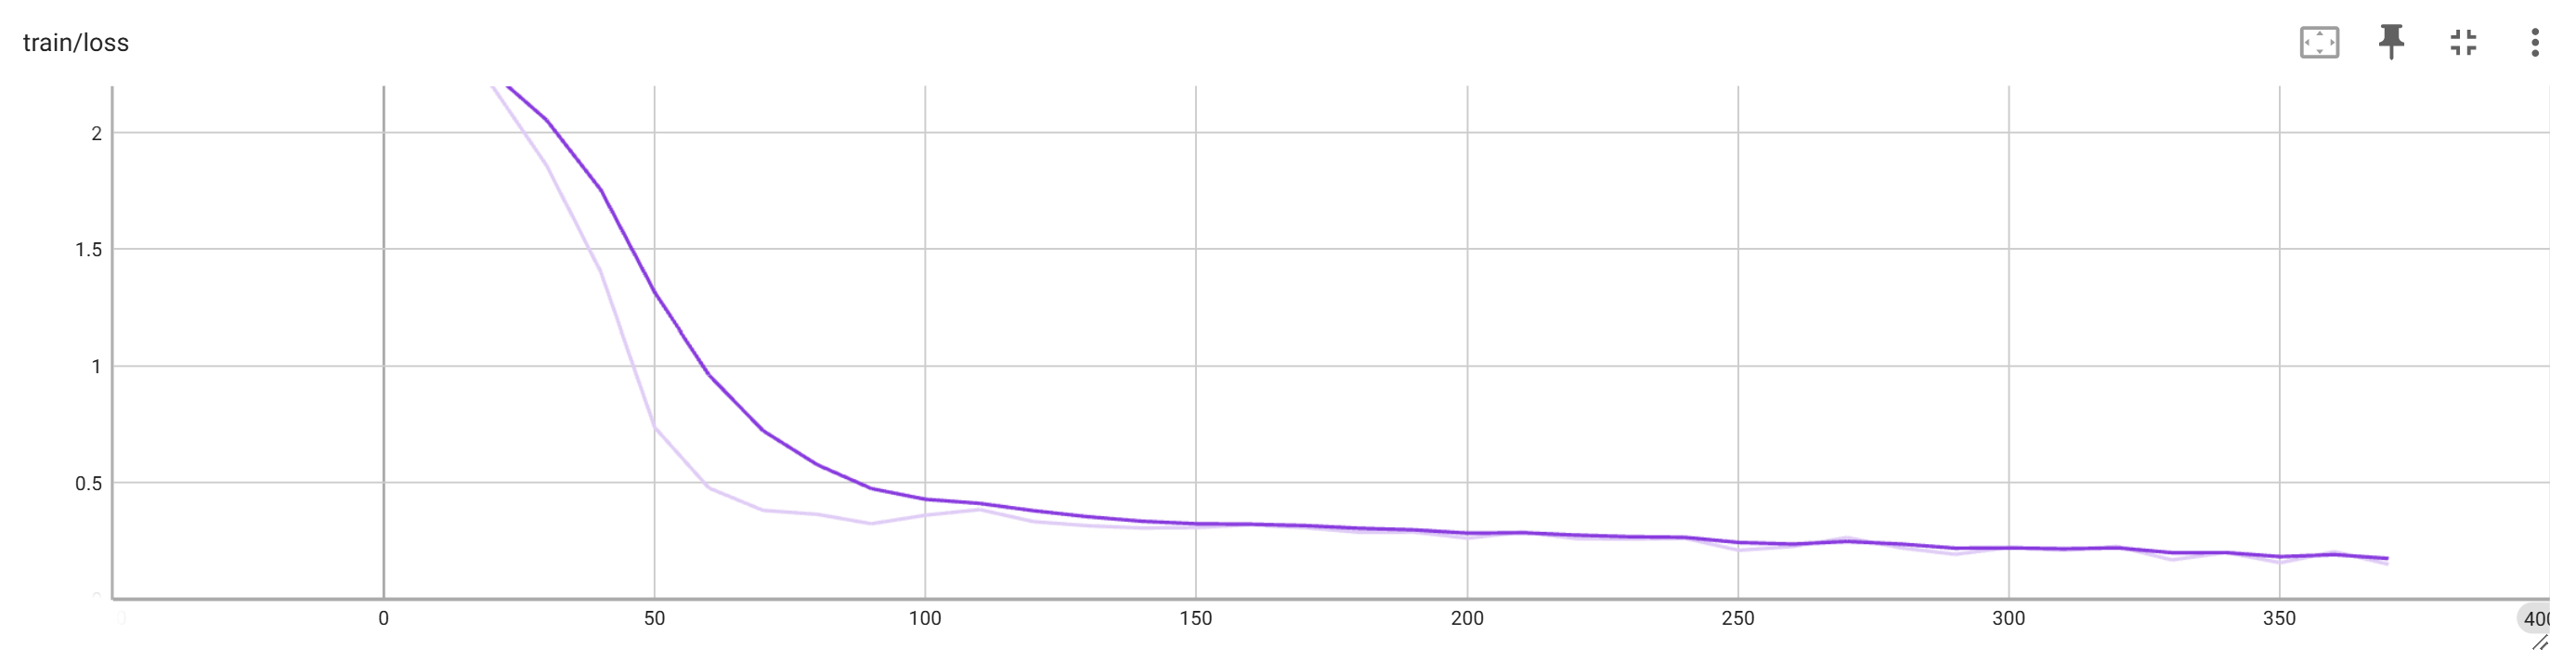
\includegraphics[width=\linewidth]{img/label_only_train_loss.png}
        \caption{Train loss}
    \end{subfigure}
    \begin{subfigure}[b]{0.49\linewidth}
        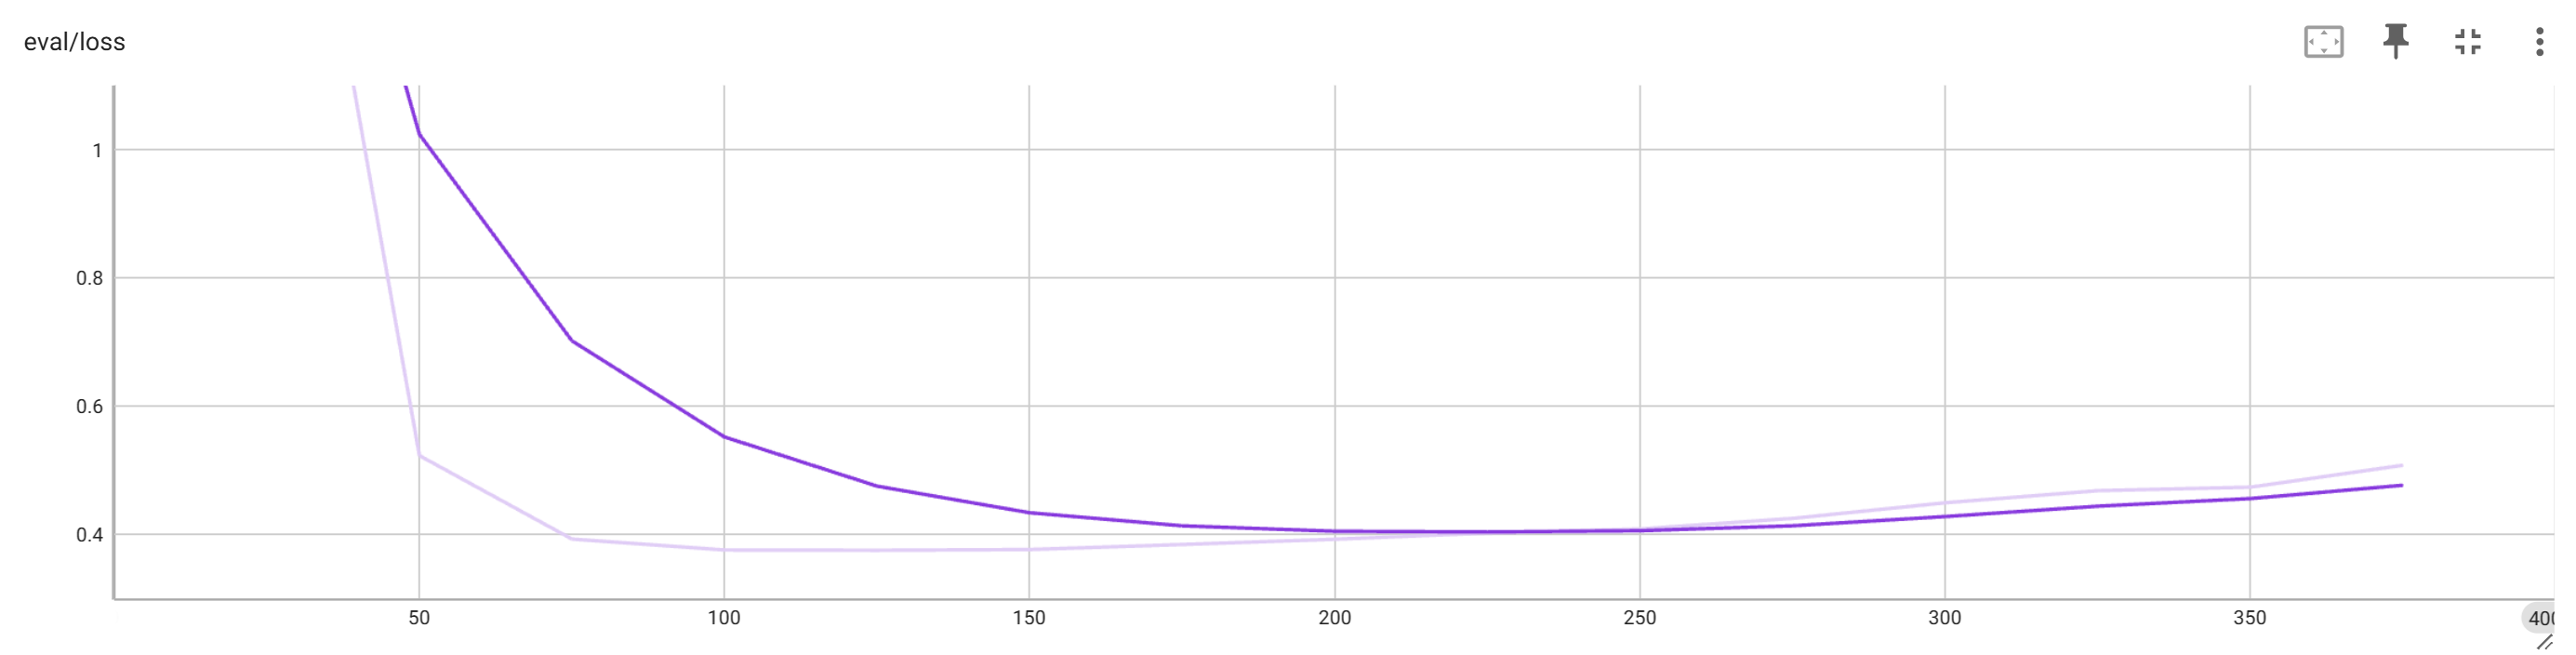
\includegraphics[width=\linewidth]{img/label_only_eval_loss.png}
        \caption{Eval loss}
    \end{subfigure}
    \caption{Label-only losses: rapid early train loss compression; eval loss reaches minimum near 180--220 steps then rises (overfitting onset).}
    \label{fig:labelonly-losses}
\end{figure}

\begin{figure}[!h]
    \centering
    \begin{subfigure}[b]{0.49\linewidth}
        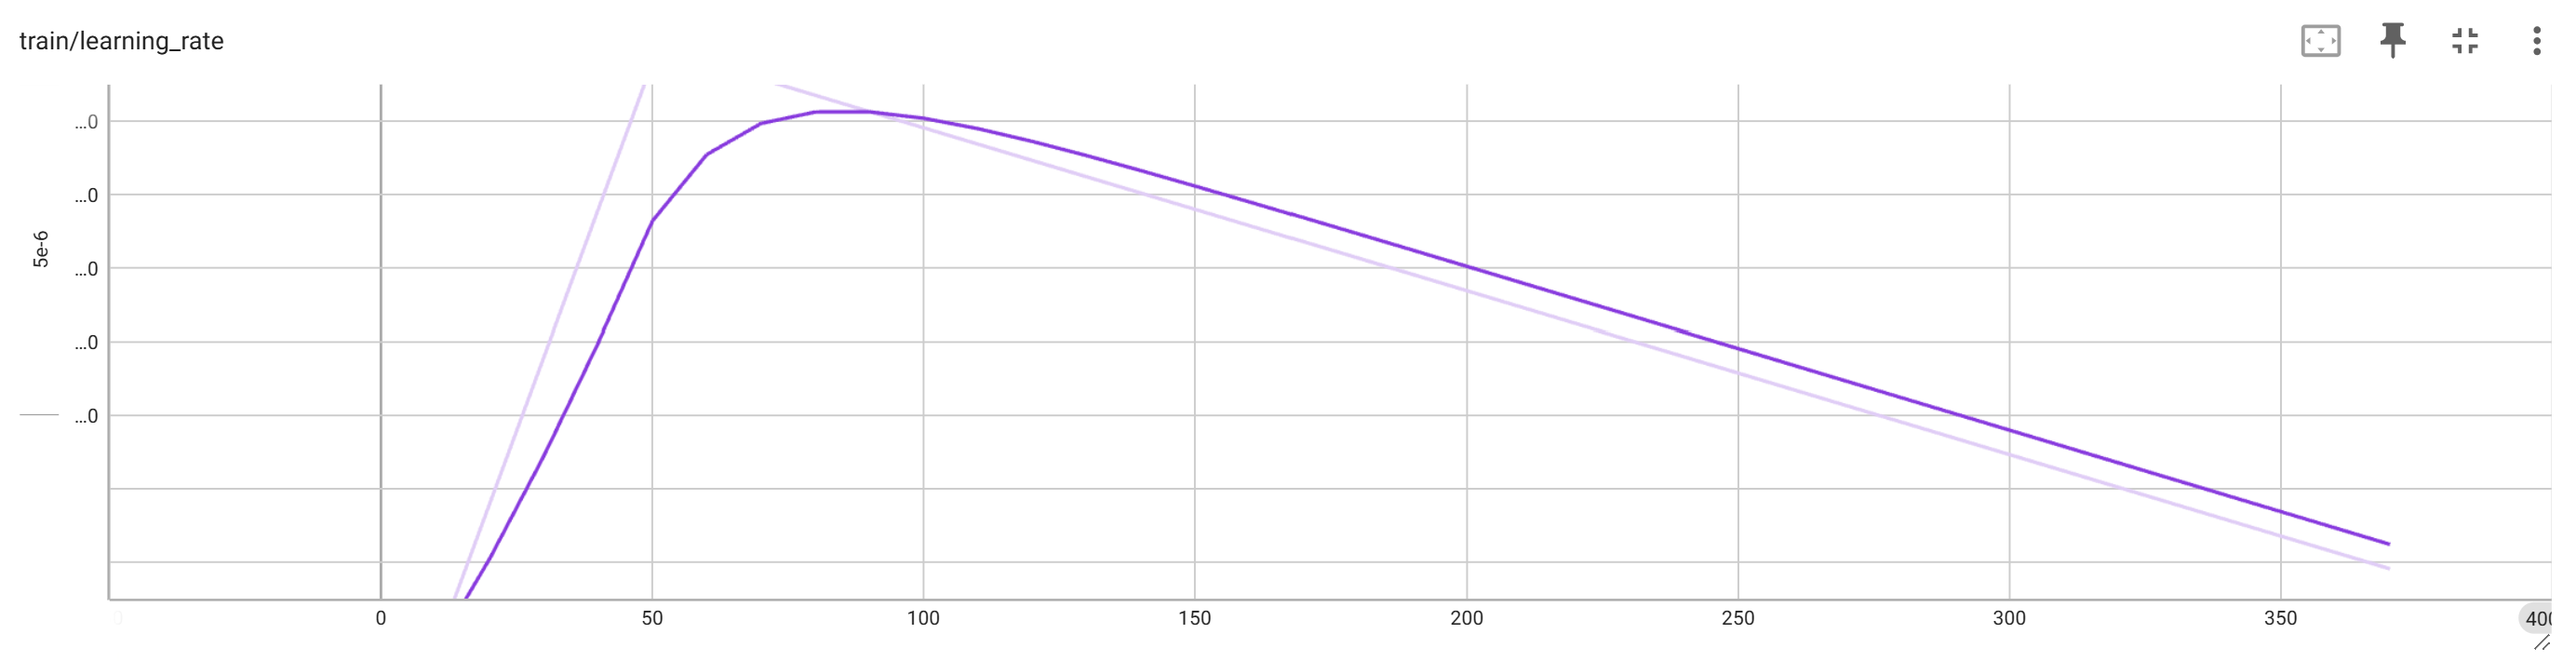
\includegraphics[width=\linewidth]{img/label_only_train_learning_rate.png}
        \caption{Learning rate}
    \end{subfigure}
    \begin{subfigure}[b]{0.49\linewidth}
        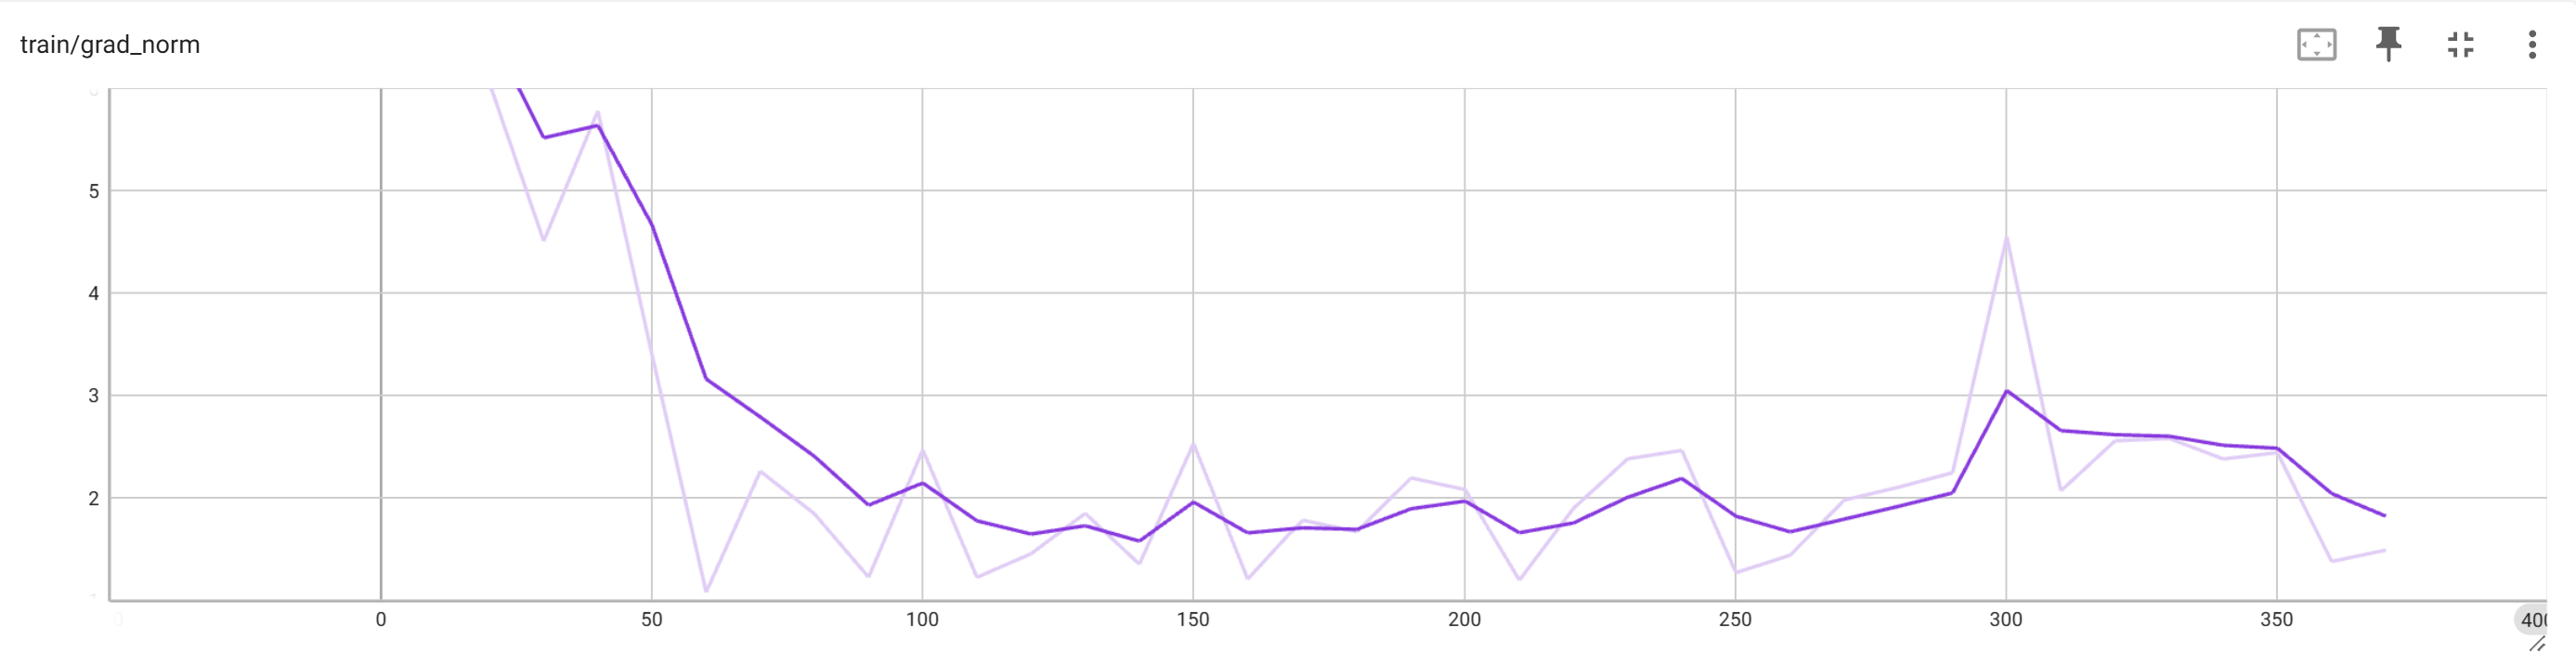
\includegraphics[width=\linewidth]{img/label_only_train_grad_norm.png}
        \caption{Grad norm}
    \end{subfigure}
    \caption{Label-only optimization dynamics: warmup then linear LR decay; early high gradient norms (>6) collapse to a stable 1.5--2.5 band.}
    \label{fig:labelonly-dynamics}
\end{figure}

Observations:
\begin{itemize}
    \item Rapid optimization: train loss drops >75\% within first \~120 steps (Figure \ref{fig:labelonly-losses}a).
    \item Generalization peak: eval loss minimum near 180--220 steps (Figure \ref{fig:labelonly-losses}b) aligns with best accuracy (15.01\%); subsequent rise indicates overfitting on formatting/token patterns.
    \item Gradient norm collapse: large initial adaptation (Figure \ref{fig:labelonly-dynamics}b) precedes eval loss floor; post-collapse stability reflects limited sequence length.
\end{itemize}

\subsection{SCoTD mode (rationale + answer)}
\begin{figure}[!h]
    \centering
    \begin{subfigure}[b]{0.49\linewidth}
        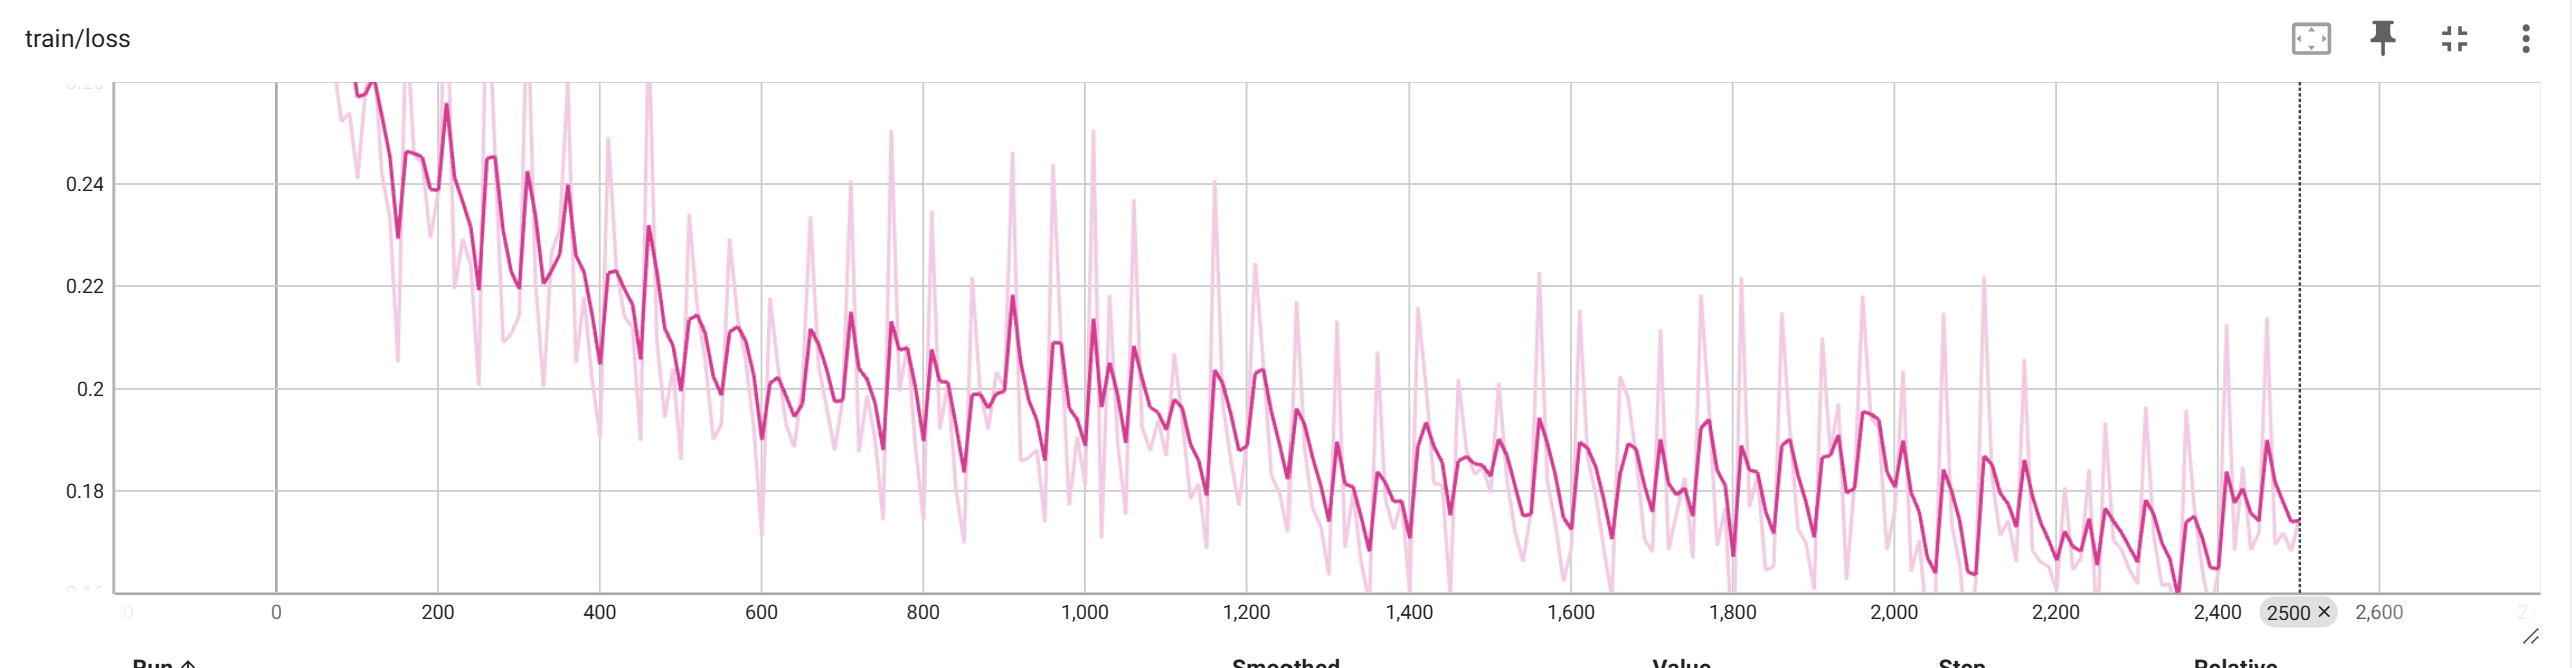
\includegraphics[width=\linewidth]{img/sctod_train_loss.png}
        \caption{Train loss}
    \end{subfigure}
    \begin{subfigure}[b]{0.49\linewidth}
        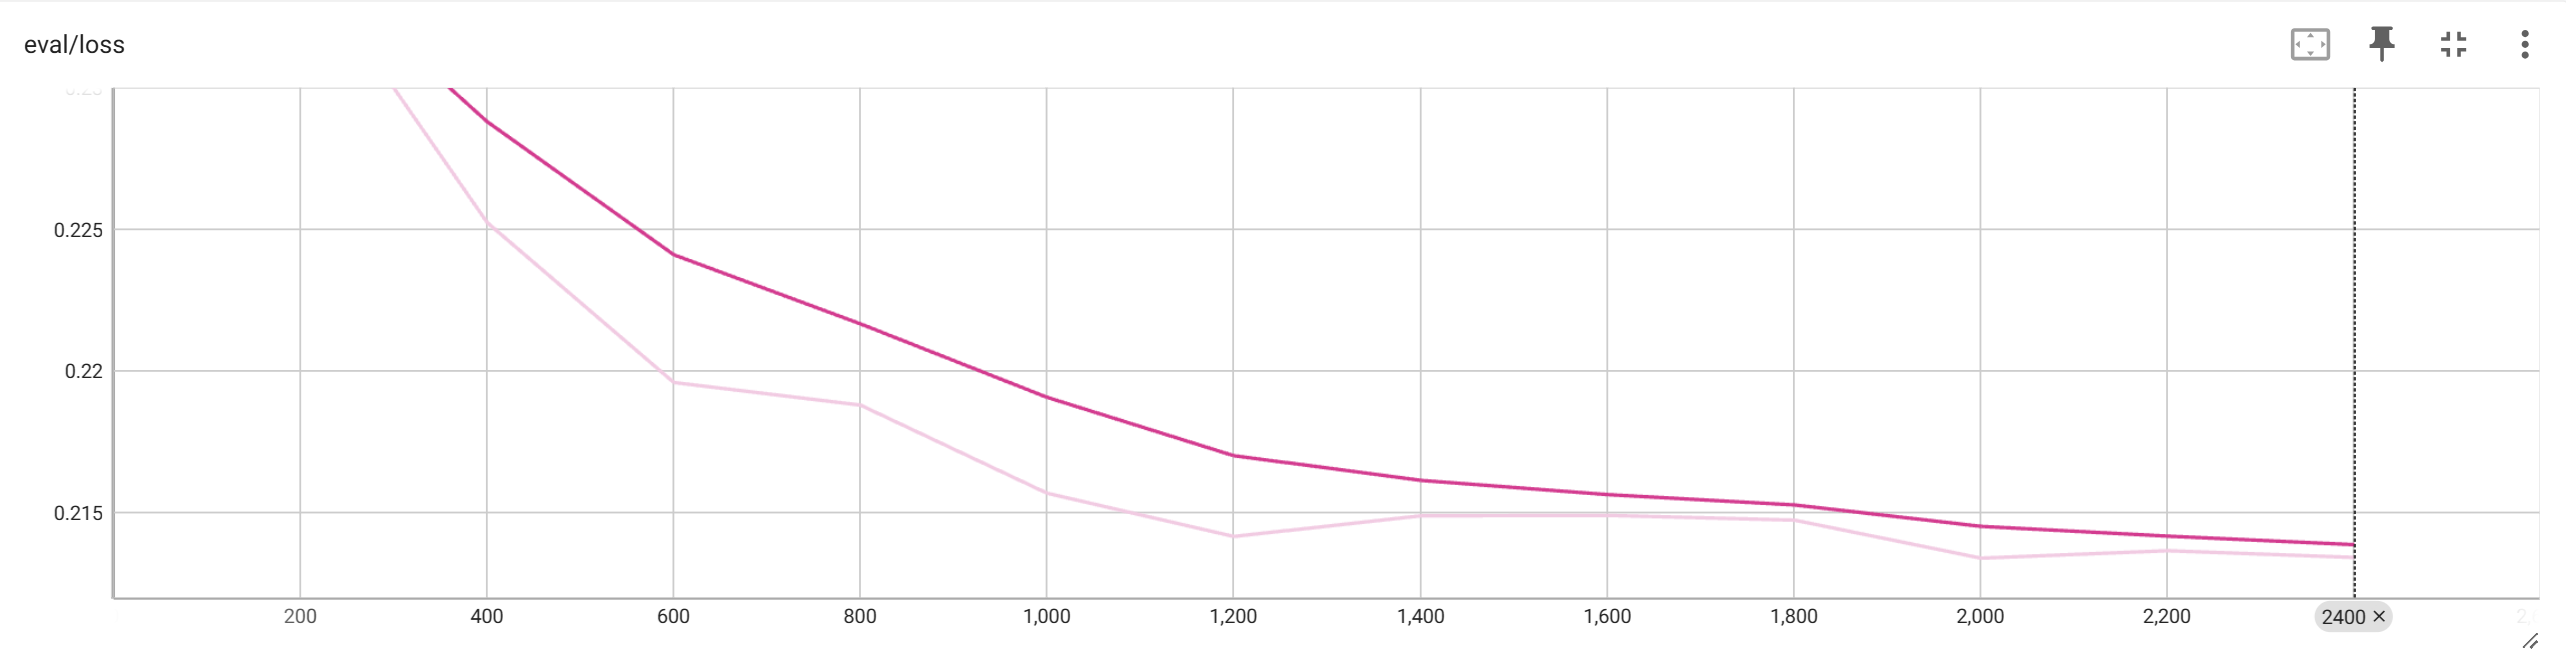
\includegraphics[width=\linewidth]{img/sctod_eval_loss.png}
        \caption{Eval loss}
    \end{subfigure}
    \caption{SCoTD losses: steady train loss descent; eval loss monotonically declines without early reversal.}
    \label{fig:sctod-losses}
\end{figure}

\begin{figure}[!h]
    \centering
    \begin{subfigure}[b]{0.49\linewidth}
        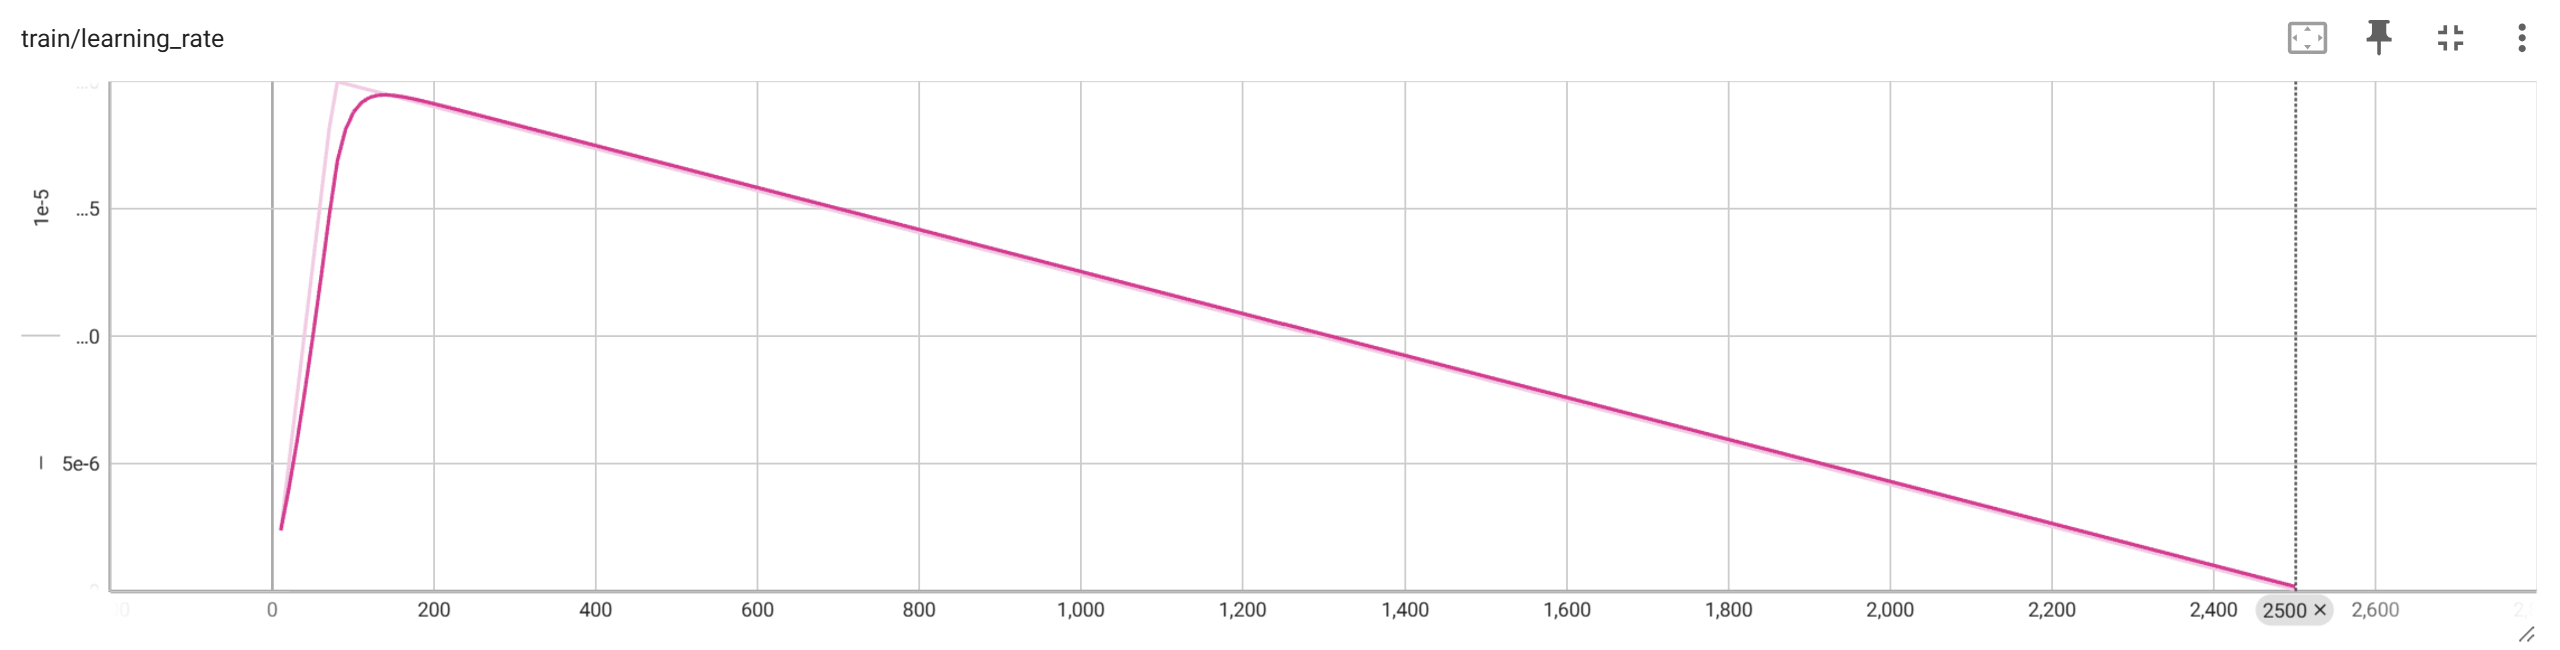
\includegraphics[width=\linewidth]{img/sctod_train_learning_rate.png}
        \caption{Learning rate}
    \end{subfigure}
    \begin{subfigure}[b]{0.49\linewidth}
        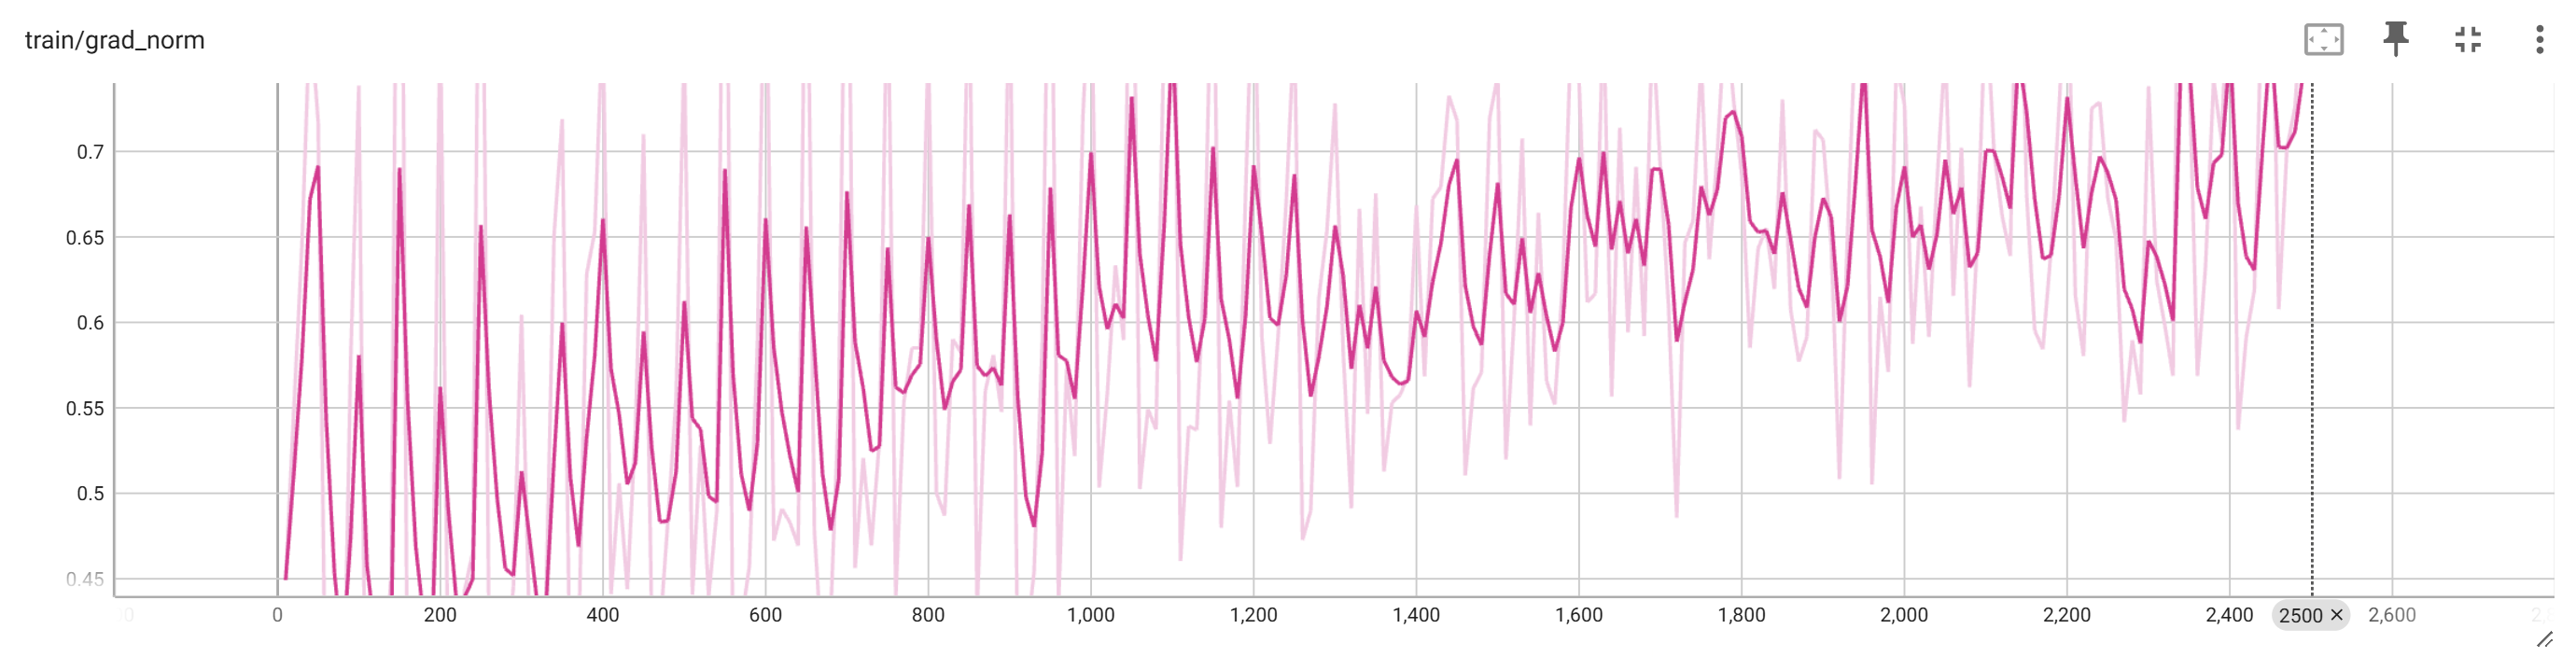
\includegraphics[width=\linewidth]{img/sctod_train_grad_norm.png}
        \caption{Grad norm}
    \end{subfigure}
    \caption{SCoTD dynamics: short warmup then linear LR decay; grad norms in a tight 0.45--0.75 band with slight late drift upward.}
    \label{fig:sctod-dynamics}
\end{figure}

Observations:
\begin{itemize}
    \item Stable optimization: absence of large spikes (Figure \ref{fig:sctod-dynamics}b) due to longer sequences distributing updates.
    \item Continued eval improvement: eval loss still falling past best accuracy checkpoint (Figure \ref{fig:sctod-losses}b) implying accuracy saturation before token-level optimum.
    \item Low variance: constrained grad norm range suggests consistent convergence; rationale diversity did not destabilize training.
\end{itemize}

\subsection{Comparison}
\begin{itemize}
    \item Label-only: faster early loss reduction (Figure \ref{fig:labelonly-losses}a) but earlier generalization peak and overfitting (Figure \ref{fig:labelonly-losses}b).
    \item SCoTD: sustained eval loss improvement (Figure \ref{fig:sctod-losses}b); accuracy plateau likely reflects reasoning ceiling rather than overfitting.
    \item Gradient behavior: high initial label-only norms (Figure \ref{fig:labelonly-dynamics}b) vs. SCoTD’s moderate steady norms (Figure \ref{fig:sctod-dynamics}b) indicate incremental adaptation with longer rationales.
\end{itemize}

\section{Output length and latency distributions}
\begin{figure}[!h]
    \centering
    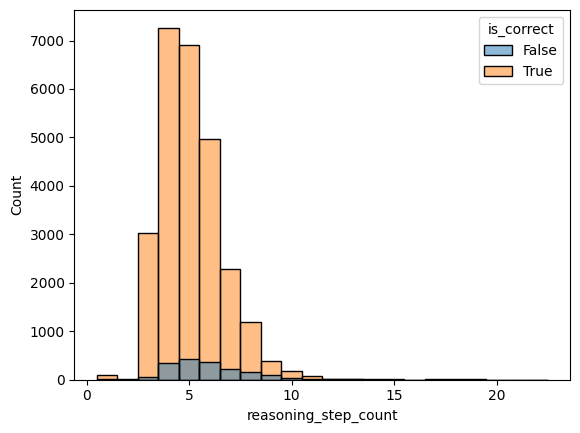
\includegraphics[width=0.48\linewidth]{img/reasoning_step_count_histogram.png}
    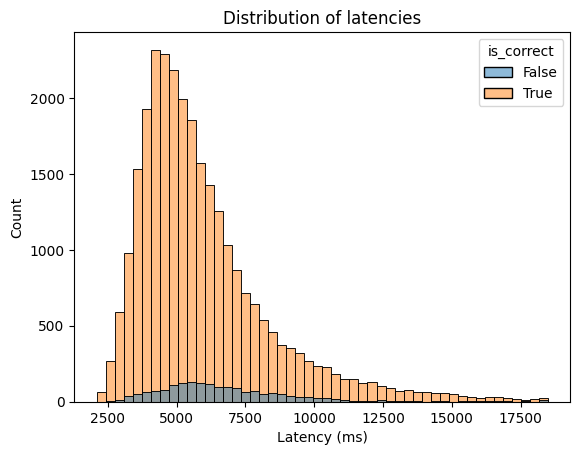
\includegraphics[width=0.48\linewidth]{img/latencies_histogram.png}
    \caption{Left: reasoning step count (mode 5, most in [4,7], rare long tails >12). Right: latency distribution (median \~5.4s, long right tail to >18s).}
    \label{fig:steps-latency}
\end{figure}

\begin{figure}[!h]
    \centering
    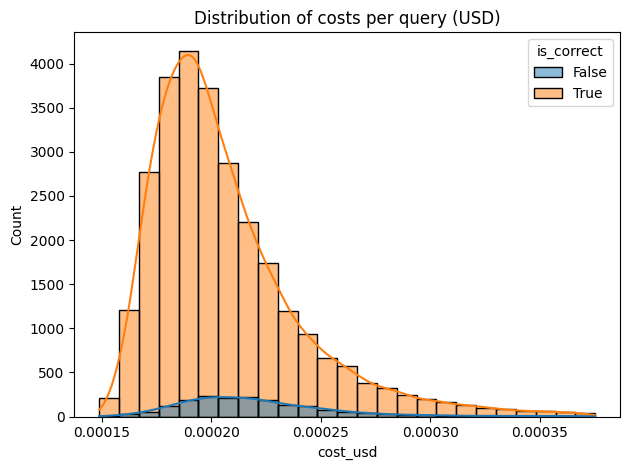
\includegraphics[width=0.295\linewidth]{img/cost_per_query_histogram.png}
    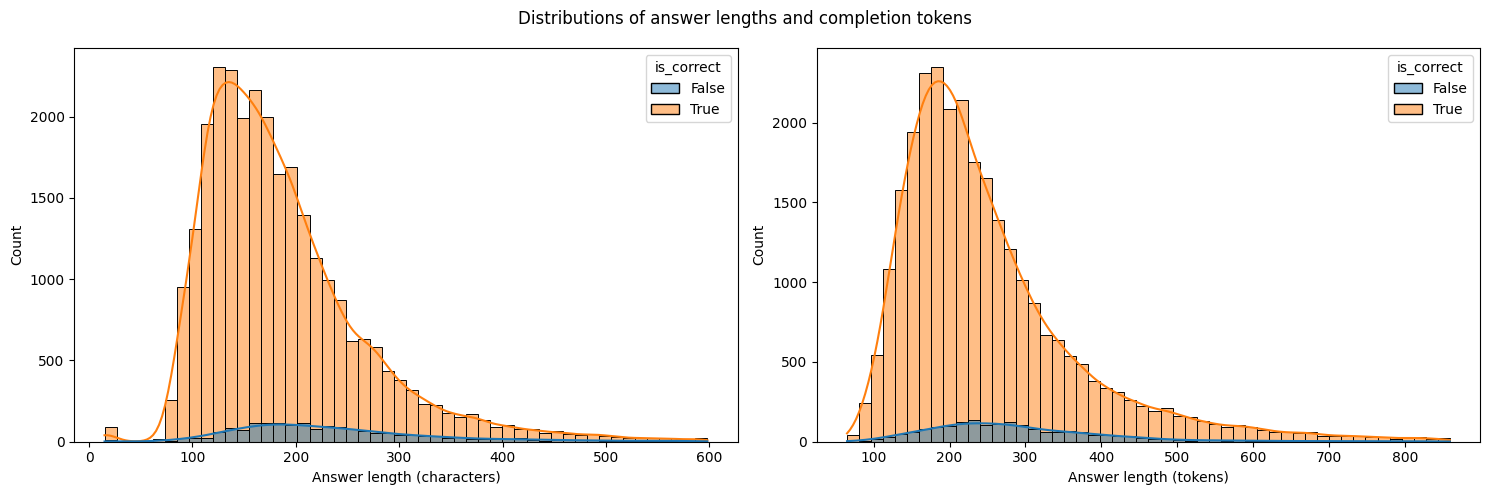
\includegraphics[width=0.685\linewidth]{img/answer_lengths_and_completion_token_histograms.png}
    \caption{Left: cost per query (right-skew, peak near \$0.00019--0.00021). Right: answer length distributions (characters and tokens; token mode \~180, tail >800).}
    \label{fig:cost-length}
\end{figure}

Quantitative summaries:
\begin{itemize}
    \item Step count: 90\% within 4--7 steps; incorrect samples slightly over-represented at 4--5 steps (shorter reasoning).
    \item Latency: interquartile band concentrated between \~4.3s and \~7.1s; heavy tail aligns with longest completions.
    \item Cost: distribution approximates log-normal; long tail beyond \$0.00030 mainly verbose rationales.
    \item Length: character median \~150; token median 225 (matches earlier quantiles); incorrect answers mildly skew shorter (information insufficiency).
\end{itemize}

\section{Dataset filtering outcomes}
\subsection{Raw and cleaned sizes}
\begin{itemize}
    \item Raw generated samples: 30{,}000 (1{,}000 train questions $\times$ 30 teacher generations).
    \item Teacher overall numeric correctness (raw): 93.75\% (28{,}125 correct).
    \item Cleaned samples retained: 24{,}952 (100\% correct after filtering).
\end{itemize}

\subsection{Removal breakdown (approximate)}
\begin{itemize}
    \item Incorrect answers removed: 1{,}875.
    \item Length outliers (>\,99th percentile total tokens; threshold $\approx$1{,}392): $\sim$300 (at most 1\%).
    \item Exact duplicate rationales removed: $\sim$2{,}873 (difference after accounting for outliers). 
\end{itemize}
Note: Duplicate vs outlier counts are approximate; precise tallies depend on overlapping removal cases.

\subsection{Effect}
Filtering ensures zero label noise and improved rationale diversity while capping worst-case sequence length for memory stability.

\section{Cost analysis}
\subsection{Aggregate}
\begin{itemize}
    \item Total teacher generation cost: \$6.33240.
    \item Average cost per raw query: \$0.00021 (median \$0.00020; std \$0.000062).
    \item Cost per retained cleaned sample: \$6.33240 / 24{,}952 $\approx$ \$0.000254.
\end{itemize}

\subsection{Distribution}
Histogram shows a right-skew with a long tail up to $\sim$\$0.00037 (Figure: cost per query). Tail samples correspond to longer completions (higher completion token counts). Tight clustering around \$0.00020 indicates stable prompt length and moderate variance in rationale length.

	\chapter{Discussion}

\section{Interpretation of quantitative outcomes}
The distilled student (78.54\% accuracy) improves over the base CoT-prompted model (70.51\%) by +8.03 percentage points under strict greedy evaluation. This gain indicates that supervised chain-of-thought distillation (SCoTD) successfully transfers structured multi-step reasoning patterns rather than merely formatting habits. The teacher at 93.61\% establishes remaining headroom: even after distillation the student closes only about 35\% of the gap to the teacher (absolute difference 23.10 points). Label-only fine-tuning produces a smaller +4.02 point improvement (15.01\% vs 10.99\%), reflecting that (i) training only the final answer line provides limited signal for intermediate decomposition, and (ii) strict formatting magnifies penalties for subtle deviations.

\section{Role of dataset filtering}
The cleaned dataset (24{,}952 samples, 100\% numerically correct) removes incorrect answers, near-duplicate rationales, and extreme-length outliers. Eliminating label noise prevents the student from learning wrong numeric terminations; rationale deduplication reduces gradient redundancy and broadens reasoning variety; length capping protects memory while retaining core arithmetic trajectories. The monotonic eval loss decline in SCoTD training suggests the filtering did not over-prune diversity needed for generalization.

\section{Training dynamics and generalization}
Label-only mode shows rapid early optimization, an early eval loss floor, and overfitting signs after \~200 steps, consistent with short targets and limited supervision richness. SCoTD exhibits slower but steadier improvement: eval loss continues decreasing past the best accuracy checkpoint, implying a saturation of accuracy before full convergence of token-level modeling. This mismatch indicates that incremental gains in reproducing teacher phrasing beyond a certain point do not translate into additional numeric correctness under greedy decoding.

\section{Formatting sensitivity}
Strict parsing (exact ``Final Answer: <number>'') penalizes:
\begin{itemize}
    \item Additional commentary after the numeric token.
    \item Missing prefix or variant capitalization.
    \item Multiple numeric candidates on the line.
\end{itemize}
The observed low label-only accuracy relative to intuitive difficulty of many questions suggests a non-trivial fraction of outputs may contain correct numbers with minor formatting deviations (not separately quantified—future work should measure the formatting error rate). This evaluation design intentionally preserves a hard constraint to highlight robustness rather than lenient post-processing.

\section{Cost and efficiency implications}
Teacher generation cost \$6.33 produced a high-signal corpus enabling a one-time accuracy gain that permanently reduces inference-time API spend. The test-set teacher cost estimate (\$0.282) contrasts with the student’s negligible marginal cost (local greedy decode). Thus, SCoTD shifts expenditure forward (data collection + training) to amortize savings over repeated evaluations. Oversampling (30 CoTs/question) proved feasible and economically justified given low per-sample cost (\$0.00021 mean).

\section{Limitations}
\begin{itemize}
    \item Single dataset (GSM8K) restricts external validity; reasoning domains with more symbolic complexity (algebraic manipulation, formal proofs) may demand different supervision properties.
    \item Single backbone (Qwen2.5-3B) prevents assessing scale effect or architectural sensitivity (e.g., mixture-of-experts, higher-rank attention).
    \item No exploration of self-consistency decoding \cite{wang2023selfconsistencyimproveschainthought} at inference; potential additive gains remain unmeasured.
    \item No ablation on filtering stages (e.g., retaining some incorrect but diverse rationales) to quantify trade-off between purity and diversity.
    \item Formatting error rate not isolated; lack of tolerant or multi-metric evaluation (e.g., relaxed number matching, rationale quality scoring).
\end{itemize}

\section{Threats to validity}
\begin{itemize}
    \item \textbf{Data contamination}: Unverified overlap of teacher pretraining data with GSM8K could inflate teacher correctness; mitigation: use official test split and public model, but provenance uncertainty remains.
    \item \textbf{Random seed dependence}: Single-seed runs may mask variance in adapter training; confidence intervals absent.
    \item \textbf{Hardware-specific behavior}: 4-bit quantization stability can vary across GPU architectures; results obtained on RTX 4090 may not exactly reproduce on other devices.
    \item \textbf{Parser rigidity}: Strict final-line parser potentially underestimates true numeric capability, especially for label-only.
    \item \textbf{Checkpoint selection bias}: Choosing best eval-loss checkpoint may not maximize accuracy if loss continues decreasing after accuracy plateau; strategy was accuracy-based (step 1400 SCoTD), minimizing this threat but still single-criterion.
\end{itemize}

\section{Implications}
\begin{itemize}
    \item High-quality filtered CoTs enable a small model to internalize multi-step arithmetic decomposition without increasing inference latency.
    \item Parameter-efficient fine-tuning (LoRA + QLoRA) is sufficient to encode reasoning gains on a single commodity GPU, reinforcing PEFT viability for resource-constrained deployments.
    \item Rationale supervision offers better return than answer-only supervision for math word problems under greedy decoding; intermediate structure is a critical training signal.
    \item Evaluation protocol design (strict formatting) materially impacts measured accuracy; downstream applications requiring reliability should incorporate format validation loops or structured decoding.
\end{itemize}

\section{Comparison to literature}
Observed gains align with symbolic CoT distillation reports \cite{li2024symbolicchainofthoughtdistillationsmall}, supporting the importance of multiple rationales per question. Difference from token/logit distillation paradigms \cite{hinton2015distilling,gou2021survey} is that sequence-level supervised rationale reproduction alone suffices for measurable reasoning improvement at small scale. The pipeline demonstrates integration of QLoRA \cite{dettmers2023qloraefficientfinetuningquantized} with multi-step reasoning tasks and confirms memory efficiency without compromising accuracy trajectory.

\section{Future work}
\begin{itemize}
    \item Quantify formatting vs numeric error decomposition to refine evaluation and potentially apply lightweight post-formatting corrections.
    \item Introduce self-consistency sampling for the distilled student to assess marginal gains beyond greedy decoding.
    \item Multi-dataset extension (e.g., SVAMP, AQuA) to evaluate cross-domain generalization of distilled reasoning.
    \item Ablation of filtering (keep partial incorrect rationales) to examine whether limited noise improves robustness or harms accuracy.
    \item Hybrid loss with partial token-level KL to teacher logits where available, combining rationale supervision with softened distribution alignment.
    \item Curriculum ordering (short → long rationales) to test whether sequence length progression affects convergence speed or final accuracy.
\end{itemize}

	\chapter{Conclusion}

The thesis investigated whether symbolic chain-of-thought distillation (SCoTD) can improve a 3B-class small language model's math reasoning accuracy on GSM8K under strict greedy evaluation. It further compared rationale+answer supervision to answer-only (label-only) fine-tuning within a constrained single-GPU environment.

To address the specific research questions posed at the beginning of this thesis, the experimental results provide clear answers. Regarding \textbf{RQ1}, SCoTD improved the student from 70.51\% (base with CoT prompting) to 78.54\% (+8.03 points). Thus, supervised rationale transfer is effective for multi-step arithmetic in a 3B model under resource constraints. Regarding \textbf{RQ2}, label-only fine-tuning improved from 10.99\% to 15.01\% (+4.02 points) but remained far below SCoTD. This demonstrates that intermediate supervision is substantially more informative than final-answer-only supervision for this task and evaluation method.

The research conducted in this thesis led to the following key observations:
\begin{itemize}
    \item Distilling structured teacher reasoning traces yields significant accuracy gains without increased inference-time cost.
    \item Rationale diversity (30 generations/question) combined with correctness filtering and deduplication produces a high-signal training set.
    \item Parameter-efficient fine-tuning provides adequate adaptation capacity for reasoning improvements in small models under tight resource constraints.
    \item Strict formatting multiplies penalties for minor output deviations, especially for label-only training; evaluation design noticeably affects reported performance.
\end{itemize}

However, the study has limitations. The reliance on a single dataset and model, the absence of self-consistency decoding, and the lack of formatting error analysis limit the generalizability and depth of insights.

In conclusion, symbolic chain-of-thought distillation offers a cost-efficient method to elevate small model reasoning without reliance on large teacher inference at deployment time. Under constrained hardware, combining high-quality rationale curation with parameter-efficient fine-tuning yields meaningful accuracy gains and provides a reproducible path toward more capable small-scale reasoning systems.

\section{Future work}
Future work should address the identified gaps by extending the methodology to additional reasoning benchmarks, model sizes, and architectures. It would be beneficial to analyze the influence of formatting errors on evaluation, experiment with self-consistency decoding to measure potential performance ceilings, and test different distillation loss functions to further optimize knowledge transfer.

	% itd.
	% \appendix
	% \include{dodatekA}
	% \include{dodatekB}
	% itd.
	
	\printbibliography

\end{document}